\documentclass[hidelinks, 12pt, oneside]{article}
\usepackage{bookmark}
\usepackage{graphicx}
\usepackage{hyperref}
\graphicspath{{images/}}
\usepackage[utf8]{inputenc}
\usepackage[english]{babel}

\begin{document}
 
%titlepage
\thispagestyle{empty}
\begin{center}
\begin{minipage}{0.75\linewidth}
    \centering
    
%University logo
    
\includegraphics{UPlogo}
    \rule{0\linewidth}{0.15\linewidth}\par

%Thesis title
    {\uppercase{\Large COS 301 Mini Project\par}}
   	{\Large Top Level Integration Testing \par} 
    \vspace{1cm}
%Author's name
    {\normalsize Elana Kuun u12029522\par}
    {\normalsize Hlavutelo Maluleke u12318109\par}
    {\normalsize Estian Rosslee u12223426\par}
    {\normalsize David Breetzke u12056503\par}
    {\normalsize Sylvester Mpungane u11241617\par}
    {\normalsize Phethile Mkhabela u12097561\par}
    {\normalsize Renaldo van Dyk  u12204359\par}
    {\normalsize Antonia Michael  u13014171\par}
    {\normalsize Herman Keuris  u13037618\par}
    {\normalsize Jaco-Louis Kruger  u13025105\par}
    \vspace{1cm}
    
    \href{https://github.com/Jaco-Louis/Top-level-testing.git}{Github Repository link}\par
    \vspace{1cm}
%Date
    {\Large April 2015}
\end{minipage}
\end{center}
\clearpage

\tableofcontents

\newpage

\section{Introduction}
The testing phase of the mini project requires thorough testing of all the aspects of both systems developed. This includes both functional and non-functional aspect of the systems. The Buzz system aimed to assist users to collaborate and share knowledge with fellow students. The system was designed in order to create modules for the various functionality required, these modules needed to be integrated to create the desired system. Both systems were developed and needed to be tested. The testing of both systems will be discussed in the following sections.

\section{Testing Results}
\subsection{Top Level A Testing Results}
\subsubsection{Functional Testing}
\begin {enumerate}
\item Buzz-Spaces Module

\begin {itemize}
\item Use Cases
\begin {itemize}
\item {createBuzzSpace}\\
This is the service which enables a lecturer to create a Buzz space for a particular module they present.
\begin {itemize}
\item Pre-conditions:\\
-buzzSpaceExists (should not be able to create a duplicate buzz space) (implemented, was unable to create a space that already existed)\\
-moduleNotActive (for the current year) (not implemented, was able to create a space for a non existent module)\\
-notAuthorized (only an authorized user can create a buzz space) (not implemented, was able to create a space without signing in as a lecturer)\\

\item Post-conditions:\\
-storeBuzzSpace (persist the new buzz space)(implemented, new buzz space was reflected in system once user is returned to home page)\\
-lecturer registered on the buzz space (not implemented)\\
-lecturer assigned as administrator of the buzz space (not implemented)\\
-Create welcome message as root thread for the buzz space (not implemented)\\
\end {itemize}

\begin{figure}[h!]
  \centering
    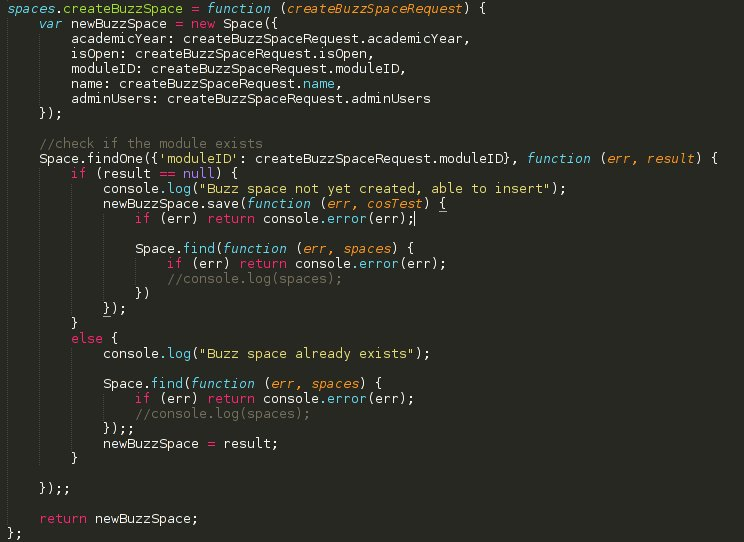
\includegraphics[width=0.85\textwidth]{buzzSpaceCreationCode} 
\end{figure}

\begin{figure}[h!]
  \centering
    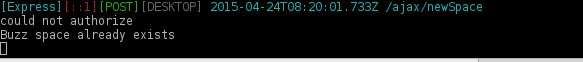
\includegraphics[width=0.85\textwidth]{buzzSpaceCreationFailToCreateDuplicate} 
\end{figure}

\begin{figure}[h!]
  \centering
    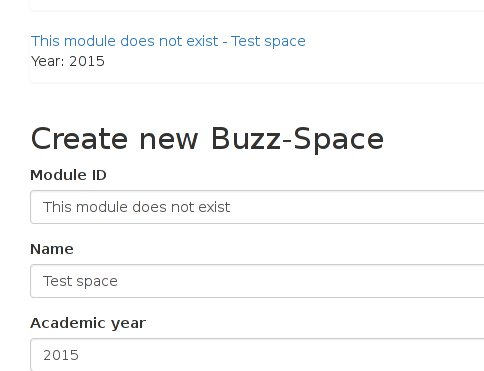
\includegraphics[width=0.85\textwidth]{buzzSpaceCreationModuleNotActive} 
\end{figure}

\begin{figure}[h!]
  \centering
    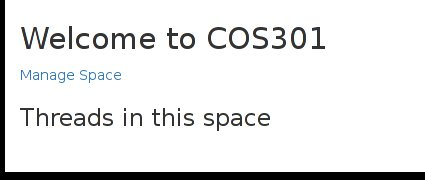
\includegraphics[width=0.85\textwidth]{buzzSpaceCreationNoRootThread} 
\end{figure}


\item {closeBuzzSpace}\\
This is the service used to set a buzz space to inactive.
\begin {itemize}
\item Pre-conditions: \\
-noSuchBuzzSpace (if buzz space to be closed does not exist then one can't close it) (was unable to find a non existent buzz space to test this)\\
        -notAuthorized (only an admin user of a buzz space can close the buzz space) (not implemented, was able to close a space I was not an admin for)\\
\item Post-conditions:\\
-buzz space no longer active (reflected upon returning to the home page)\\
\end{itemize}

\begin{figure}[h!]
  \centering
    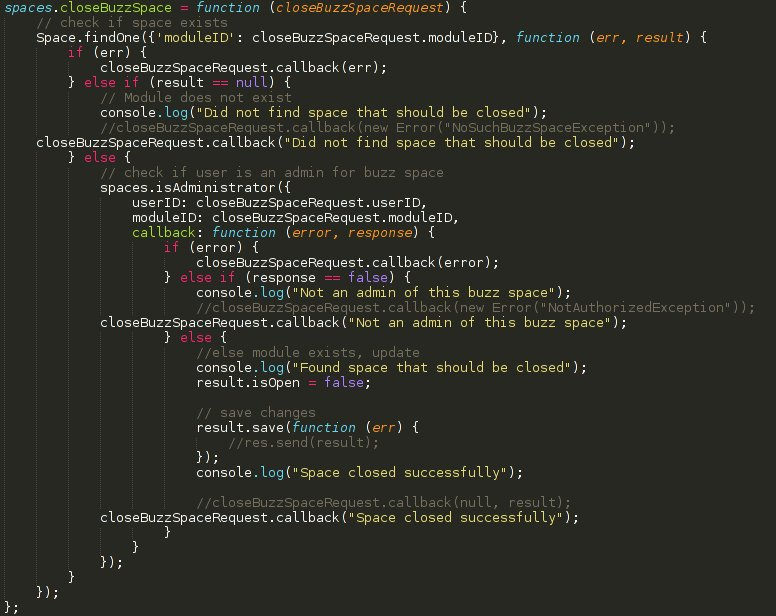
\includegraphics[width=0.85\textwidth]{buzzSpaceCloseCode} 
\end{figure}

\begin{figure}[h!]
  \centering
    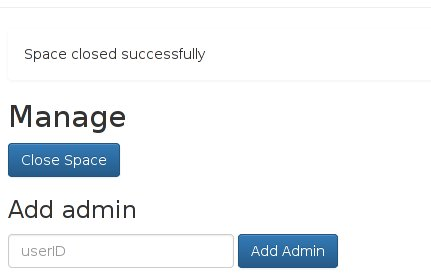
\includegraphics[width=0.85\textwidth]{buzzSpaceCloseSuccessful} 
\end{figure}

\begin{figure}[h!]
  \centering
    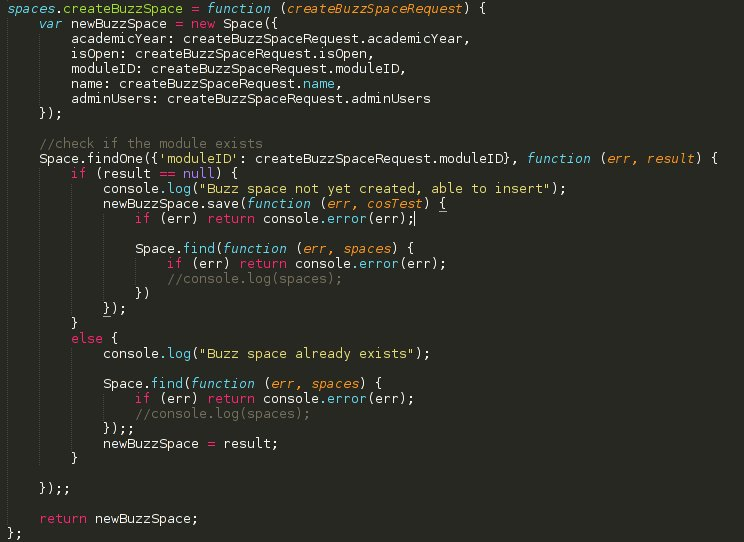
\includegraphics[width=0.85\textwidth]{buzzSpaceCreationCode} 
\end{figure}

\begin{figure}[h!]
  \centering
    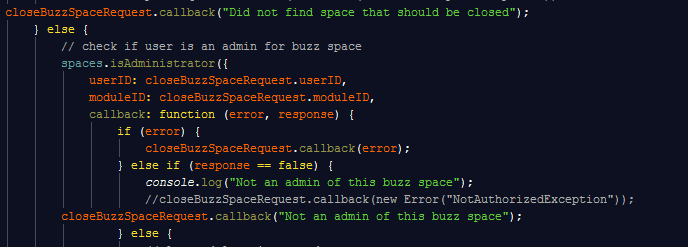
\includegraphics[width=0.85\textwidth]{closeBuzzSpace} 
\end{figure}

\item {registerOnBuzzSpace}\\
This service is used to create a profile for a user on a particular buzz space.
\begin {itemize}
\item Pre-conditions: \\
-notAuthorized (user is registered for the module to which the space is associated) (not implemented, was able to register a fake user successfully)\\
        -buzz space active (implemented, only able to access register for spaces which are active on home page)\\
\item Post-conditions: \\
 -user profile persisted to database (implemented) (screenshots provided for proof)\\
\end{itemize}

\begin{figure}[h!]
  \centering
    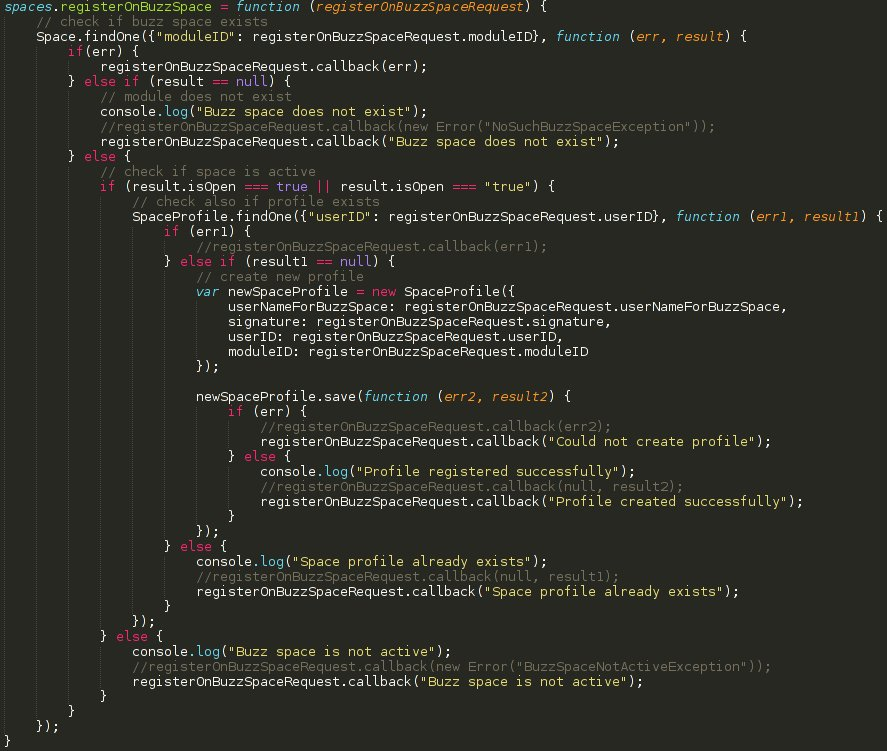
\includegraphics[width=0.85\textwidth]{buzzSpaceRegisterCode} 
\end{figure}

\begin{figure}[h!]
  \centering
    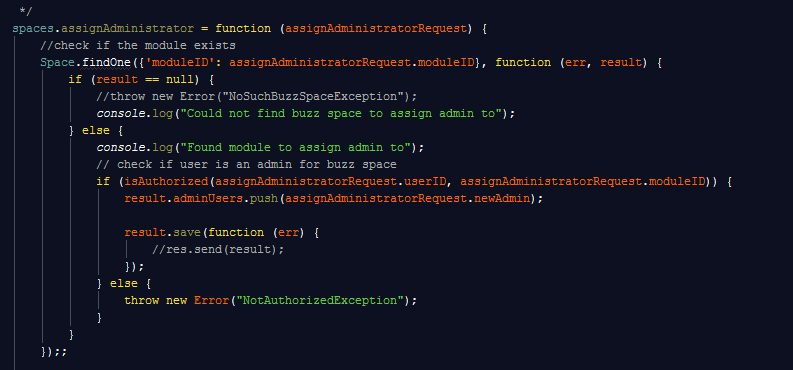
\includegraphics[width=0.85\textwidth]{addAdmin} 
\end{figure}

\item{getProfileForUser}
Simply returns the profile the user has on the buzz space\\
Code found but no functional implementation exists in the system that could be tested \\
\end{itemize}
\end{itemize}


\item Buzz-Data-Sources
\begin {itemize}
\item Use Cases
\begin {itemize}
\item {login}\\
Login - Using a provided username and password authenticates the user against details retrieved from an ldap repository
\begin {itemize}
\item Pre-conditions:\\
-could connect to CS data source (LDAP) (implemented in code only, no functional way to test)\\
        -user exists in ldap with provided authentication details (code indicates this is checked by performing a bind to ldap using the provided details)\\
\item Post-conditions:\\
userID returned (not implemented)  
\end {itemize}

\begin{figure}[h!]
  \centering
    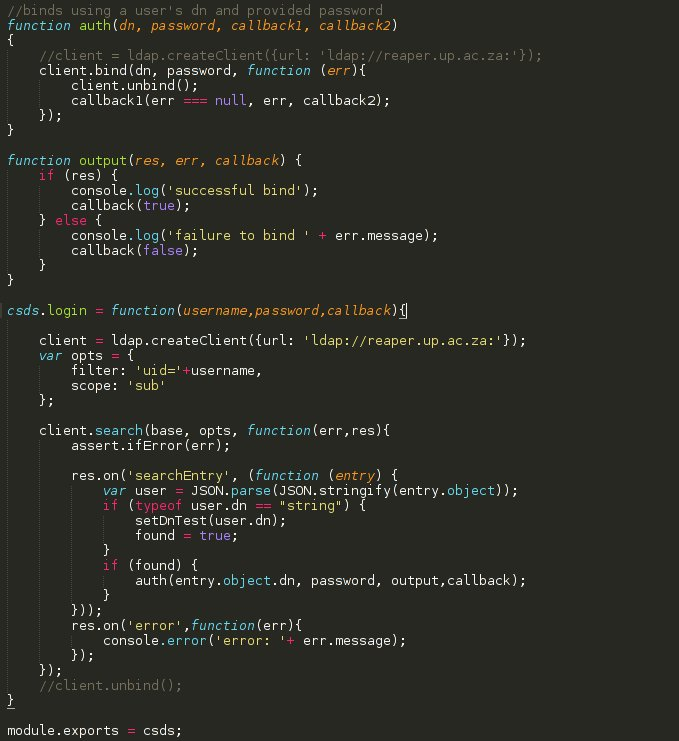
\includegraphics[width=0.85\textwidth]{CSDSLoginCode} 
\end{figure}


\end {itemize}

\begin {itemize}
\item {getUsersRolesForModule}\\
Login - Using a provided username and password authenticates the user against details retrieved from an ldap repository\\
\begin {itemize}
\item Pre-conditions:\\
-could connect to CS data source (LDAP) (implemented in code only, no functional way to test)\\
        -user exists in ldap with provided authentication details (code indicates this is checked by performing a bind to ldap using the provided details)\\
\item Post-conditions:\\
userID returned (not implemented)  
\end {itemize}
\end {itemize}

\begin {itemize}
\item {getUsersWithRole}\\
retrieves all users with a particular role for a particular module (no functional way to test)
\begin {itemize}
\item Pre-conditions:\\
-could connect to CS data source (LDAP) (implemented in code only, no functional way to test)\\  
\end {itemize}

\begin{figure}[h!]
  \centering
    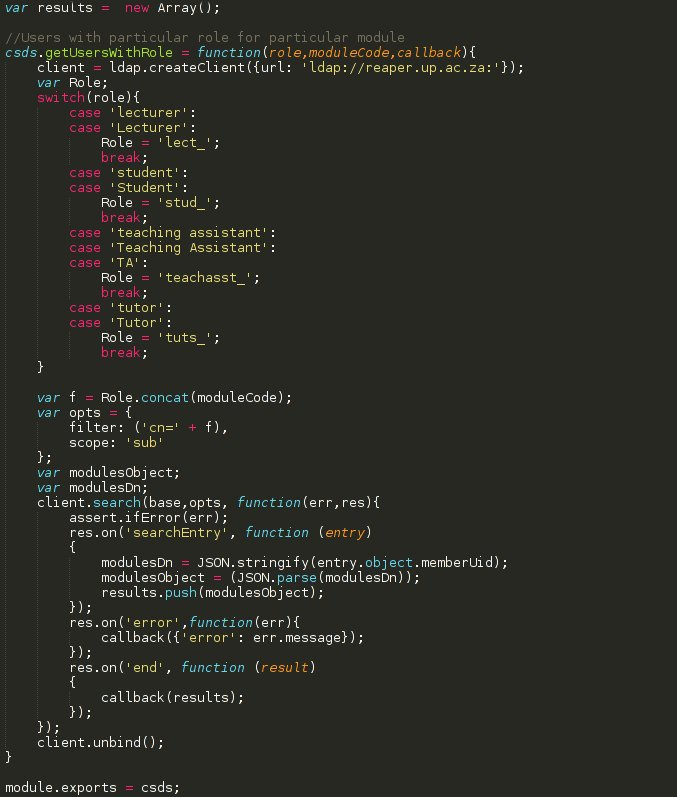
\includegraphics[width=0.85\textwidth]{CSDSGetUsersWithRolesCode} 
\end{figure}


\end {itemize}

\begin {itemize}
\item {getActiveModulesForYear}\\
retrieves all users with a particular role for a particular module (no functional way to test)
\begin {itemize}
\item Pre-conditions:\\
-could connect to CS data source (LDAP) (implemented in code only, no functional way to test)\\  
\end {itemize}
\end {itemize}

\begin {itemize}
\item {getActiveModulesForYear}\\
retrieves all users with a particular role for a particular module (no functional way to test)
\begin {itemize}
\item Pre-conditions:\\
-could connect to CS data source (LDAP) (implemented in code only, no functional way to test)\\  
\end {itemize}
\end {itemize}






\end {itemize}


\item Buzz Status
\begin {itemize}
\item Use Cases
\begin {itemize}
\item {AssessProfile}\\ 
This is where the lecturers can specify different ways to assess the students. In the current system, this functionality is not present.
SetStatusCalculator - This is where the status is calculated according to the number of posts the user has made. Again, this functionality does not exist in the sysemt and hence cannot be tested. 
\end {itemize}
 
\begin {itemize}
\item {getStatusForProfile}\\ 
This query returns status for a specific profile. 
createAppraisalType - New appraisal types are created that can be reused. The current system makes use of this functionality where a user can add appraisals under the appraisal tab on the menu bar, where an option exists to add an appraisal type.\\ The various options that exist, regarding this, is adding appraisal name, description, and adding apprasials on different levels by adding new levels with descriptors and ratings. \\
\end {itemize}

\begin {itemize}
\item {activateAppraisalType}\\ 
This use case activates an appraisal type for a specified period on a specific buzz space. This was not implemented.
\end {itemize}
\end {itemize}


\item Buzz-reporting
\begin {itemize}
\item Use Cases
\begin {itemize}
\item {getThreadStats}\\ 
Returns statistical information of subsets of posts complying with specified restrictions (code present but no functional way to test from system)\\
\end {itemize}

\begin{figure}[h!]
  \centering
    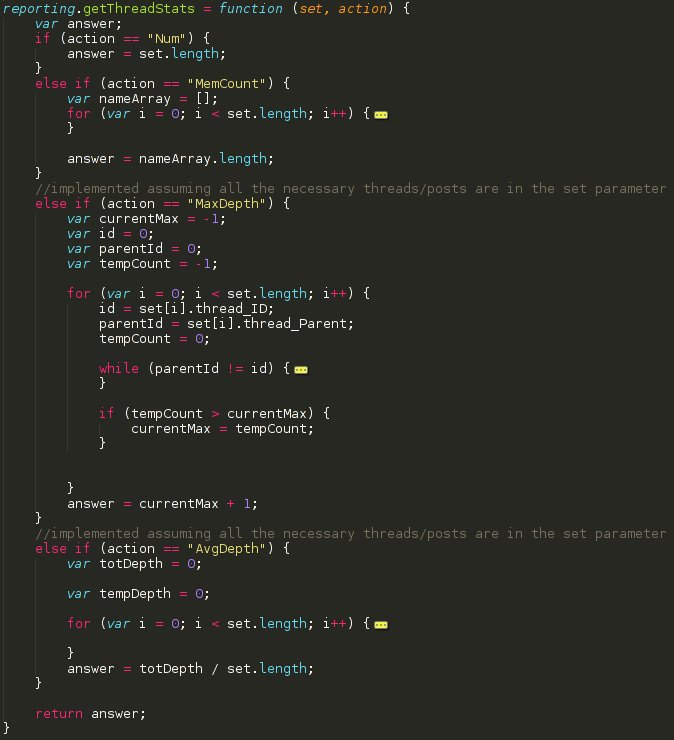
\includegraphics[width=0.85\textwidth]{buzzReportingGetThreadStatsCode} 
\end{figure}

\begin {itemize}
\item {getThreadAppraisal}\\ 
 (code not present, not implemented, not testable) \\ 
\end {itemize}

\begin {itemize}
\item {exportThreadAppraisal}\\ 
 (code not present, not implemented, not testable) \\ 
\end {itemize}

\begin {itemize}
\item {importThreadAppraisal}\\ 
 (code not present, not implemented, not testable) \\ 
\end {itemize}


\begin {itemize}
\item {exportThread}\\ 
Service to backup the content of a thread (implemented in code only, no functional way to test from system) \\ 
\end {itemize}

\begin{figure}[h!]
  \centering
    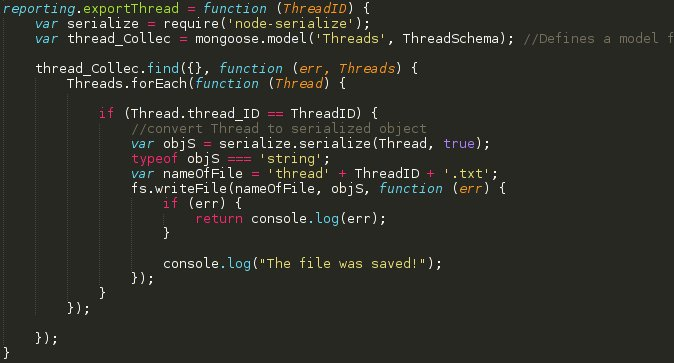
\includegraphics[width=0.85\textwidth]{buzzReportingExportThreadCode} 
\end{figure}

\begin {itemize}
\item {importThread}\\ 
Service to backup the content of a thread (implemented in code only, no functional way to test from system) \\ 
\end {itemize}

\begin{figure}[h!]
  \centering
    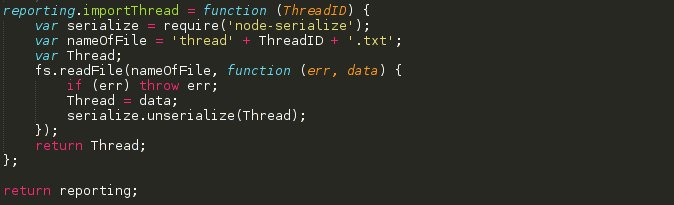
\includegraphics[width=0.85\textwidth]{buzzReportingImportThreadCode} 
\end{figure}



\end {itemize}


\end {enumerate}
 
 

\subsubsection{Non-functional Testing} 

\begin{enumerate}
\item Maintainability: 

In order for a system to be maintainable, the system should be both flexible and extensible.  For developers to continue maintenance on the system, it would require that the system should be easy to understand, the technologies used should be available for an extended period of time and developers should be able to easily add new functionality to the system. 

The code tested satisfies the condition that it should be able to understand the system. The system developed is not cluttered and difficult to understand due to good extraction between layers in the Model View Controller model. An obstacle in trying to understand the system is that the code has not been thoroughly documented. This causes some difficulties when trying to gain a better context about certain functions, why they are there and what their purposes are.

The technologies chosen satisfies the requirement of having to be available for a long period of time. The technologies used (such as Node js), are relevantly new platform and therefore they are constantly being updated. This will ensure long use of the technologies, enhancing maintainability.

Developers would be able to easily maintain the code in the sense of adding new features. This is made possible for example by making use of the simple way to add a new route to the program. There might however be slight difficulties when trying to change certain aspects of the system, due to the system being developed too specific, rather than focusing on adaptability. More emphasis was put on being able to easily add to the system, rather than changing the system, though it will still be possible it would only take longer than adding to the system.

\item Scalability:

In order for a system to be scalable, the system should be able to expand and scale in order to handle a larger load or to serve more clients. 

The system satisfies scalability in the sense that it is currently able to handle all the modules for the computer science department. This is however only a small portion of what the system should be capable of doing. The system should theoretically be able to scale in order to service 50 000 students. This should not be a problem for the system, due to the technologies that it are using. Node js is a lot more scalable than Apache, even though it is only single threaded by default. The use of MongoDB, rather than MySql also increases the scalability of the server [1].  The scalability of Node js can be increased by using multi-core CPUs rather than a single core CPU and load balancers can be implemented. This will ensure that the server application scales more than enough in order to be able to serve the required amount of users. This can however only be done when purchasing more efficient hardware for the host machine. 

\item Performance:

The performance requirements set out in the formal specification stated that all non reporting operations should respond within less than 0.2 seconds. The specification also stated that report queries should not take any longer than 5 seconds.

The performance testing was done using Firebug for Firefox. Almost all of the non reporting requests responded well under 0.1 seconds. The only cases where the server did not respond fast enough, was when the page was initially requested. The initial page request resulted in a response time of 1.33s which was the worst case. On average the initial request for the homepage resulted in about 305ms response time. 
The next case that took longer than it should, is when a page is requested that does not exist. The reason for this decrease in performance is due to the server searching for a route that does not exist. The server will then eventually just give up and return the error page. This resulted in an average response time of about 286ms. 

The overall average response time for requests is about 150ms as determined by firebug. Below are some screenshots created during the testing of non reporting requests.

The performance for the reporting use cases exceeded expectations by performing well under the recommended 5s. This might however change as the database size increases. Testing was limited to the usage of a fairly small size database. 

On average the generating of a report averaged at about 310ms. Below are some screenshots that was taken during the performance testing of the report requests. 

\begin{figure}[h!]
  \centering
    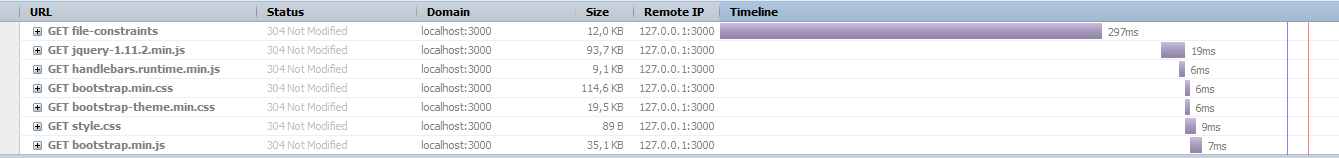
\includegraphics[width=0.85\textwidth]{performance1}
    \caption{Non reporting based request for constraints}
\end{figure}

\begin{figure}[h!]
  \centering
    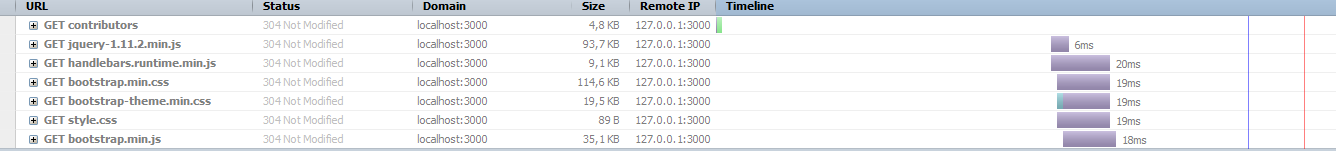
\includegraphics[width=0.85\textwidth]{performance2}
    \caption{Non reporting based request for contributors}
\end{figure}

\begin{figure}[h!]
  \centering
    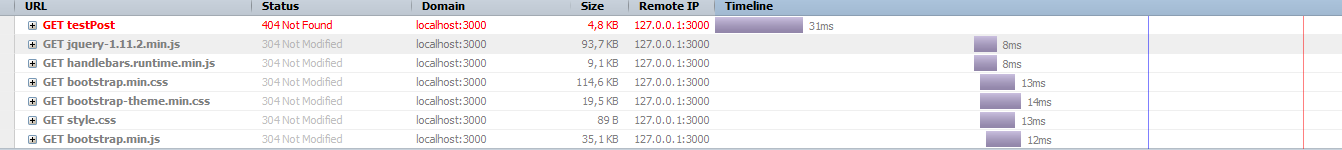
\includegraphics[width=0.85\textwidth]{performance3}
    \caption{Non reporting based request for test Post. Results in 404 error}
\end{figure}

\begin{figure}[h!]
  \centering
    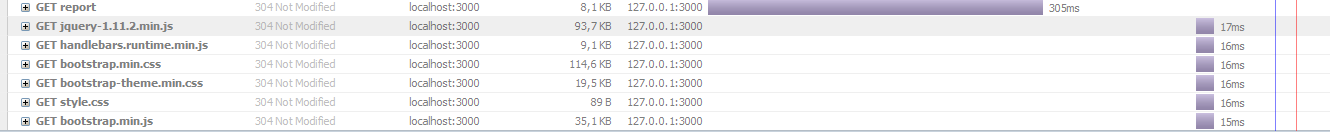
\includegraphics[width=0.85\textwidth]{performanceR1}
    \caption{Reporting based request}
\end{figure}

\begin{figure}[h!]
  \centering
    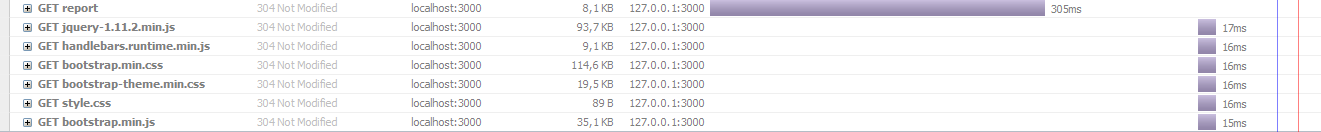
\includegraphics[width=0.85\textwidth]{performanceR2}
    \caption{Reporting based request}
\end{figure}

\begin{figure}[h!]
  \centering
    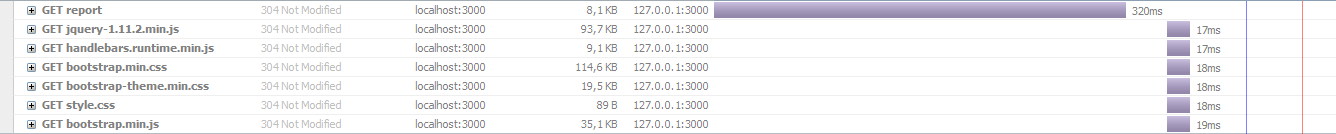
\includegraphics[width=0.85\textwidth]{performanceR3}
    \caption{Reporting based request}
\end{figure} 
 
\item Security 

The system is not secure in all areas. It requires a username and password in order for a user to login. The system successfully performs authentication against the LDAP repository. It does not allow users without the necessary authorisation to delete buzz spaces, but anyone can create a buzz space whether they are logged in or not. Only authorised users can add or remove admins. The system is also somewhat configurable, MIME types can be added, edited, and removed, but the system does not take authorisation level or whether a user is logged in into account for these actions, anyone can perform these actions. Admin users cannot configure access to certain services.

The log in user interface:

\begin{figure}[h!]
  \centering
    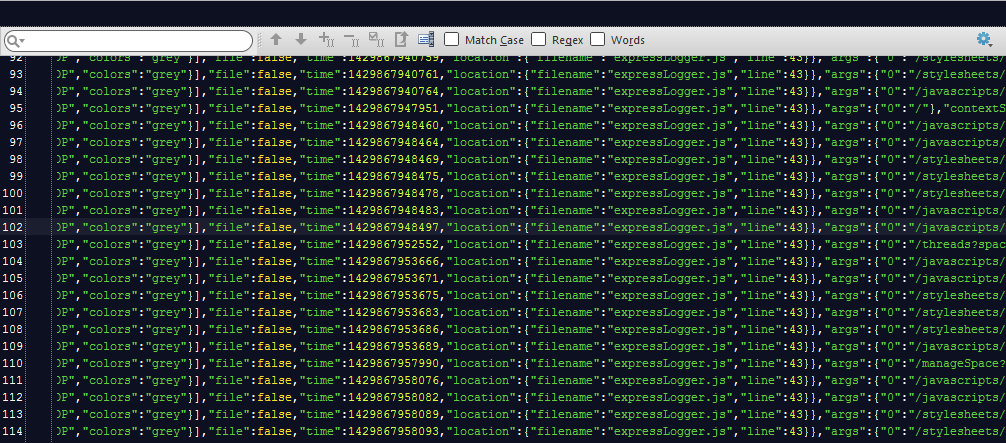
\includegraphics[width=0.85\textwidth]{logFile} 
\end{figure}

Determine if the user is authorised to close the buzz space:


\begin{figure}[h!]
  \centering
    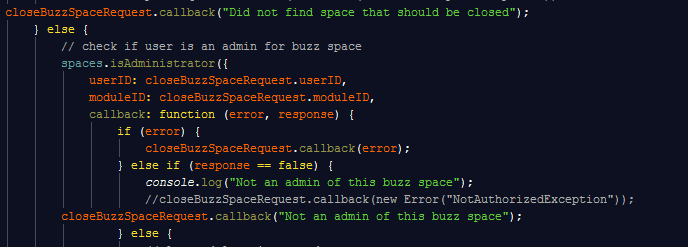
\includegraphics[width=0.85\textwidth]{closeBuzzSpace} 
\end{figure}

Assign an admin to a BuzzSpace:


\begin{figure}[h!]
  \centering
    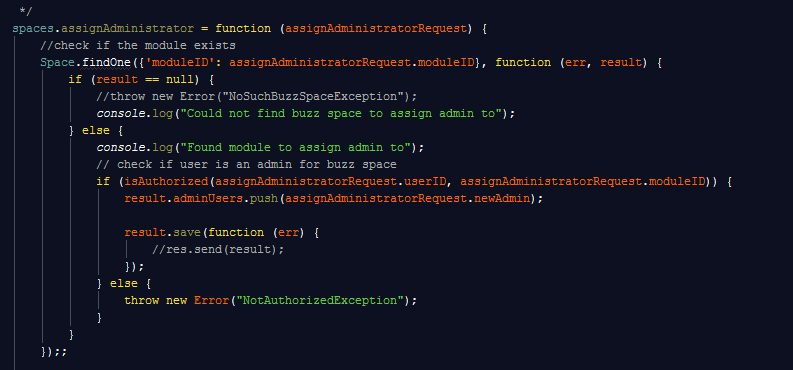
\includegraphics[width=0.85\textwidth]{addAdmin} 
\end{figure}


\item Auditability:

The system is auditable. 
The system keeps a log of all the requests and responses. The requests does not have an id, but it does have a user id, a date/time stamp, it includes the request that was made, and it does not store any sensitive information.

For the responses, there is not an id for the log entry or a corresponding request entry, there is a date/time stamp, and there is no sensitive information included. Because the response entries does not have a way of indicating to which request it responded it can be difficult to make sense of the date or to trace errors.

The audit log can be accessed by humans and the system. 


\begin{figure}[h!]
  \centering
    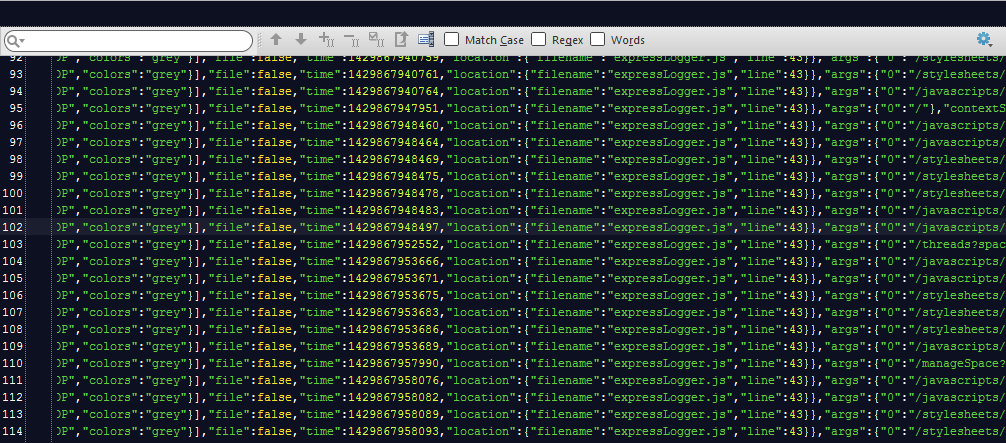
\includegraphics[width=0.85\textwidth]{logFile} 
\end{figure}

\begin{figure}[h!]
  \centering
    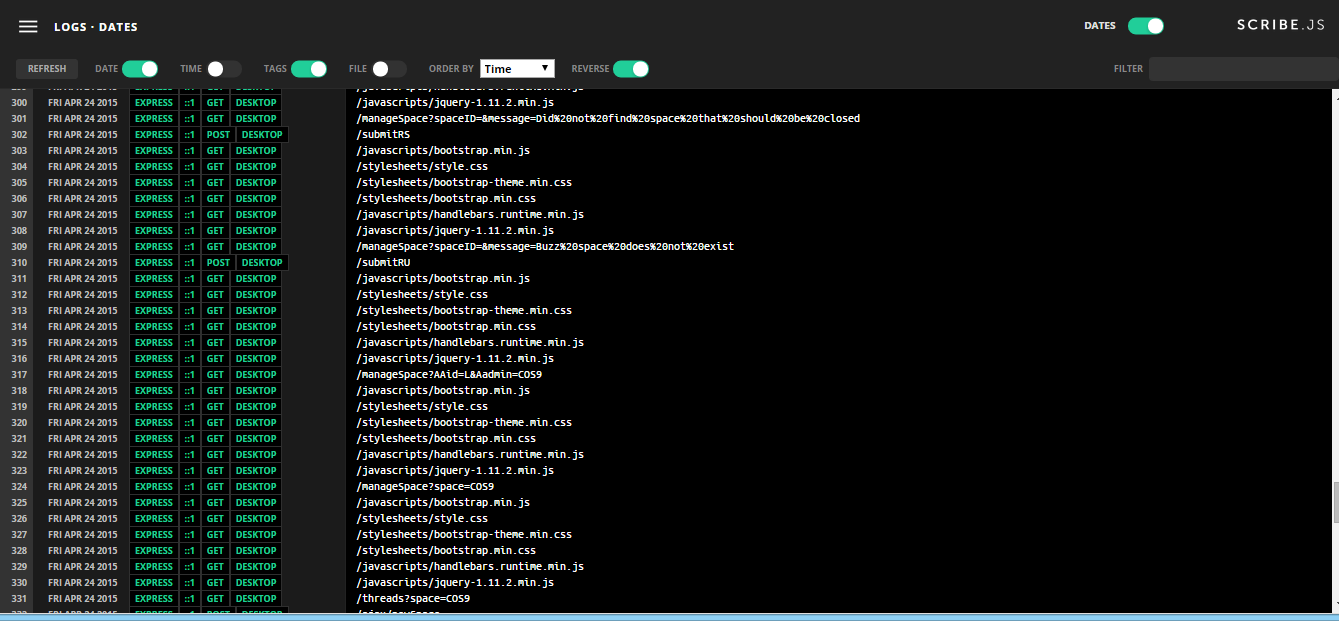
\includegraphics[width=0.85\textwidth]{logs} 
\end{figure}

An example of responses that are logged:
A buzzSpace does not exist:

\begin{figure}[h!]
  \centering
    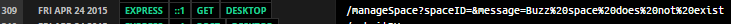
\includegraphics[width=0.85\textwidth]{buzzNotExistLog} 
\end{figure}

Could not find space to remove:

\begin{figure}[h!]
  \centering
    
\includegraphics[width=0.85\textwidth]{couldNotFindSpaceLog} 
\end{figure}

Request to manage space COS9:

\begin{figure}[h!]
  \centering
    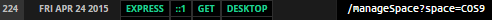
\includegraphics[width=0.85\textwidth]{manageSpaceLog} 
\end{figure}

Response that states a space was closed successfully:

\begin{figure}[h!]
  \centering
    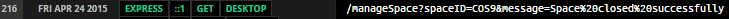
\includegraphics[width=0.85\textwidth]{ClosedSpaceLog} 
\end{figure}

\item Testability:
Only some modules included unit tests. For example, threads and spaces:
Unit testing for threads:

\begin{figure}[h!]
  \centering
    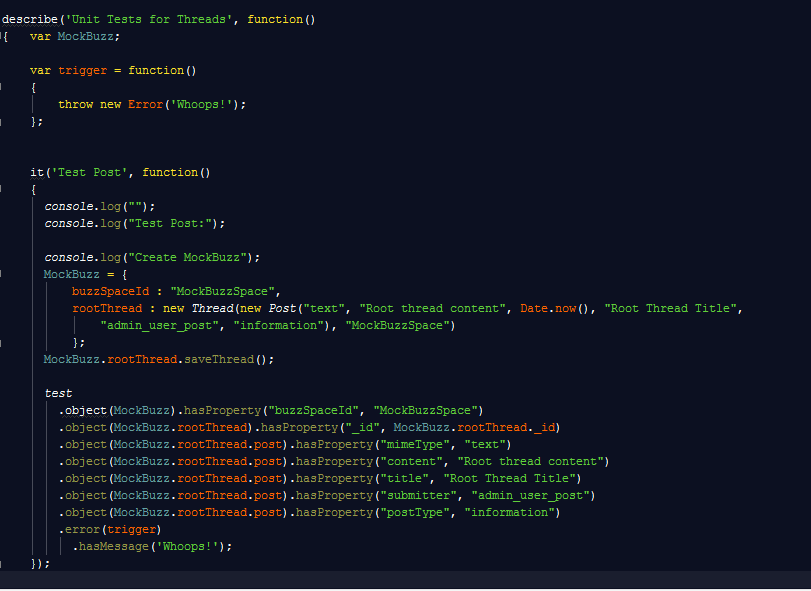
\includegraphics[width=0.85\textwidth]{unit_tests} 
\end{figure}


Integration tests are also performed in some instances. 

In this instance authorisation is checked outside of the module that is was created in.

\begin{figure}[h!]
  \centering
    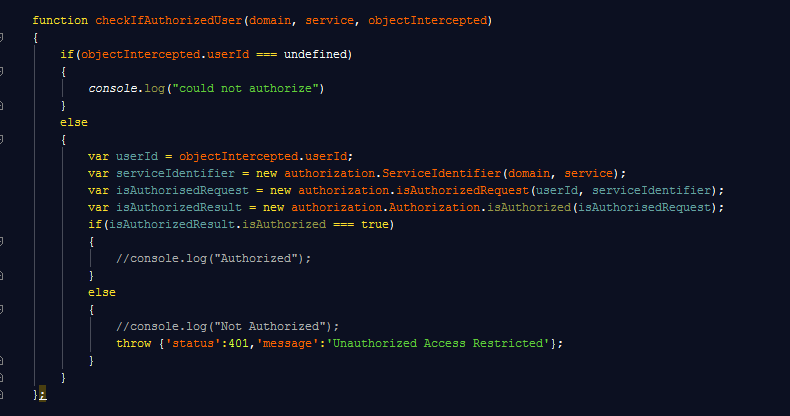
\includegraphics[width=0.85\textwidth]{integration} 
\end{figure}


For both the user tests and the integration tests it is verified that all the pre-conditions are met 

The system is thus only testable in some cases, but there is a lot of potential to add further test cases as the system is set up in such a way that makes testing more convenient.
 

\item Usability:

The system is usable because firstly the necessary actions that a user can take appear in a navigation bar at the top of the screen. Thus it is easy for a novice user to be able to know what to click on and navigate the website. 

\begin{figure}[h!]
  \centering
    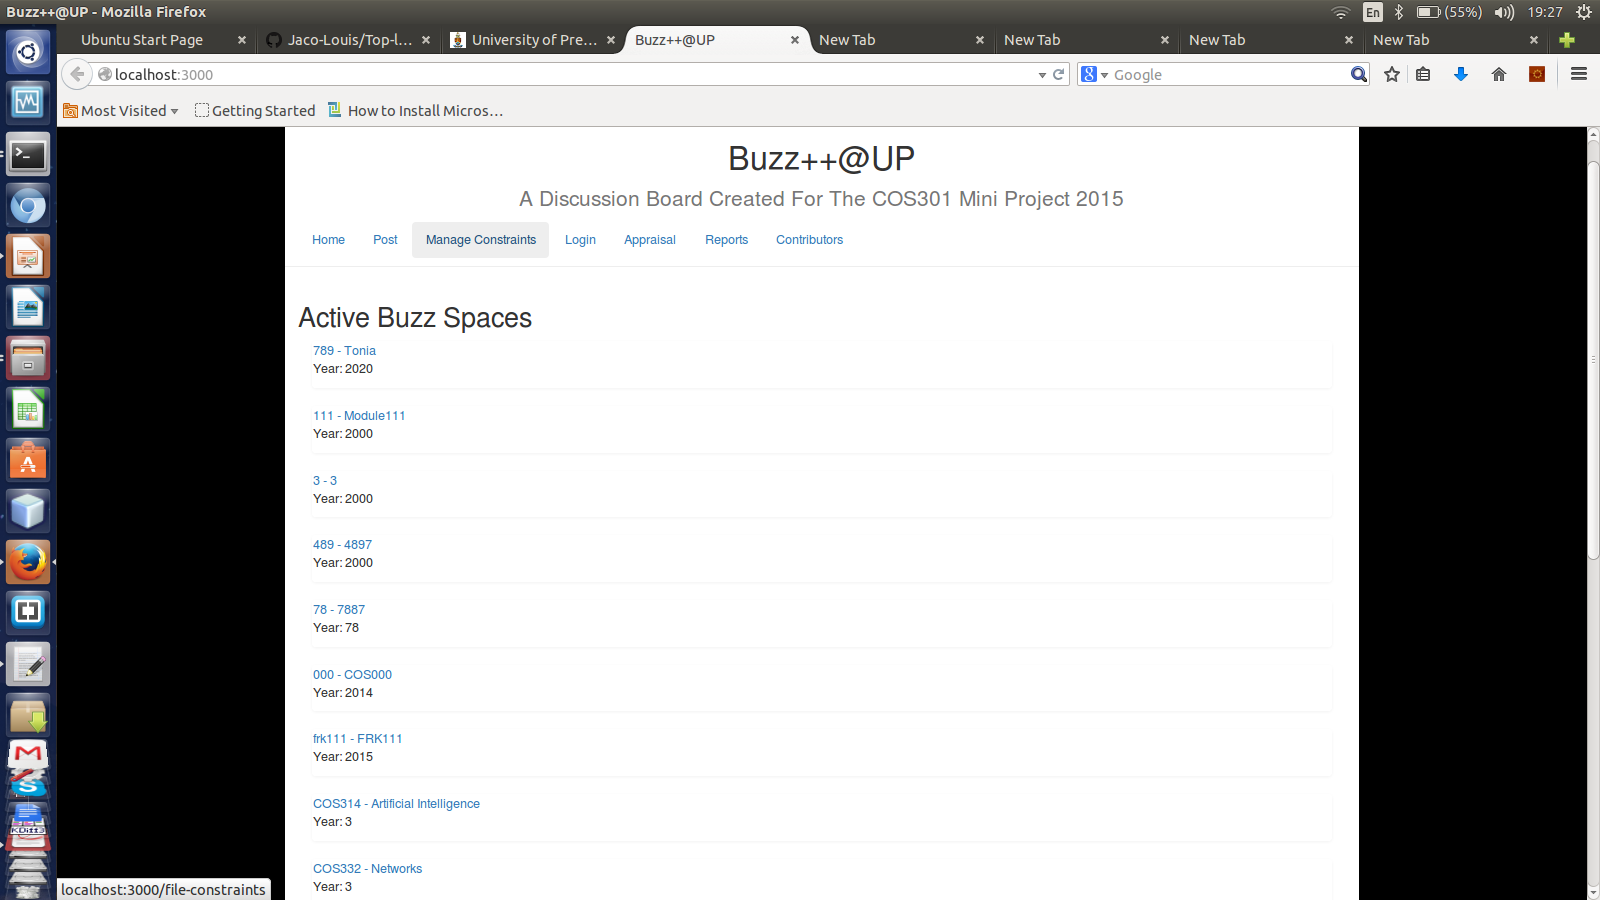
\includegraphics[width=0.85\textwidth]{UsabilityScreenshotNavBar.png} 
\end{figure}

The interface is not cluttered, and only basic functionality is displayed on the home screen, making the system more learnable. The buttons are labelled with text rather than with graphical icons, and the text on the button is quite explanatory, which makes their purpose more clear. 

\begin{figure}[h!]
  \centering
    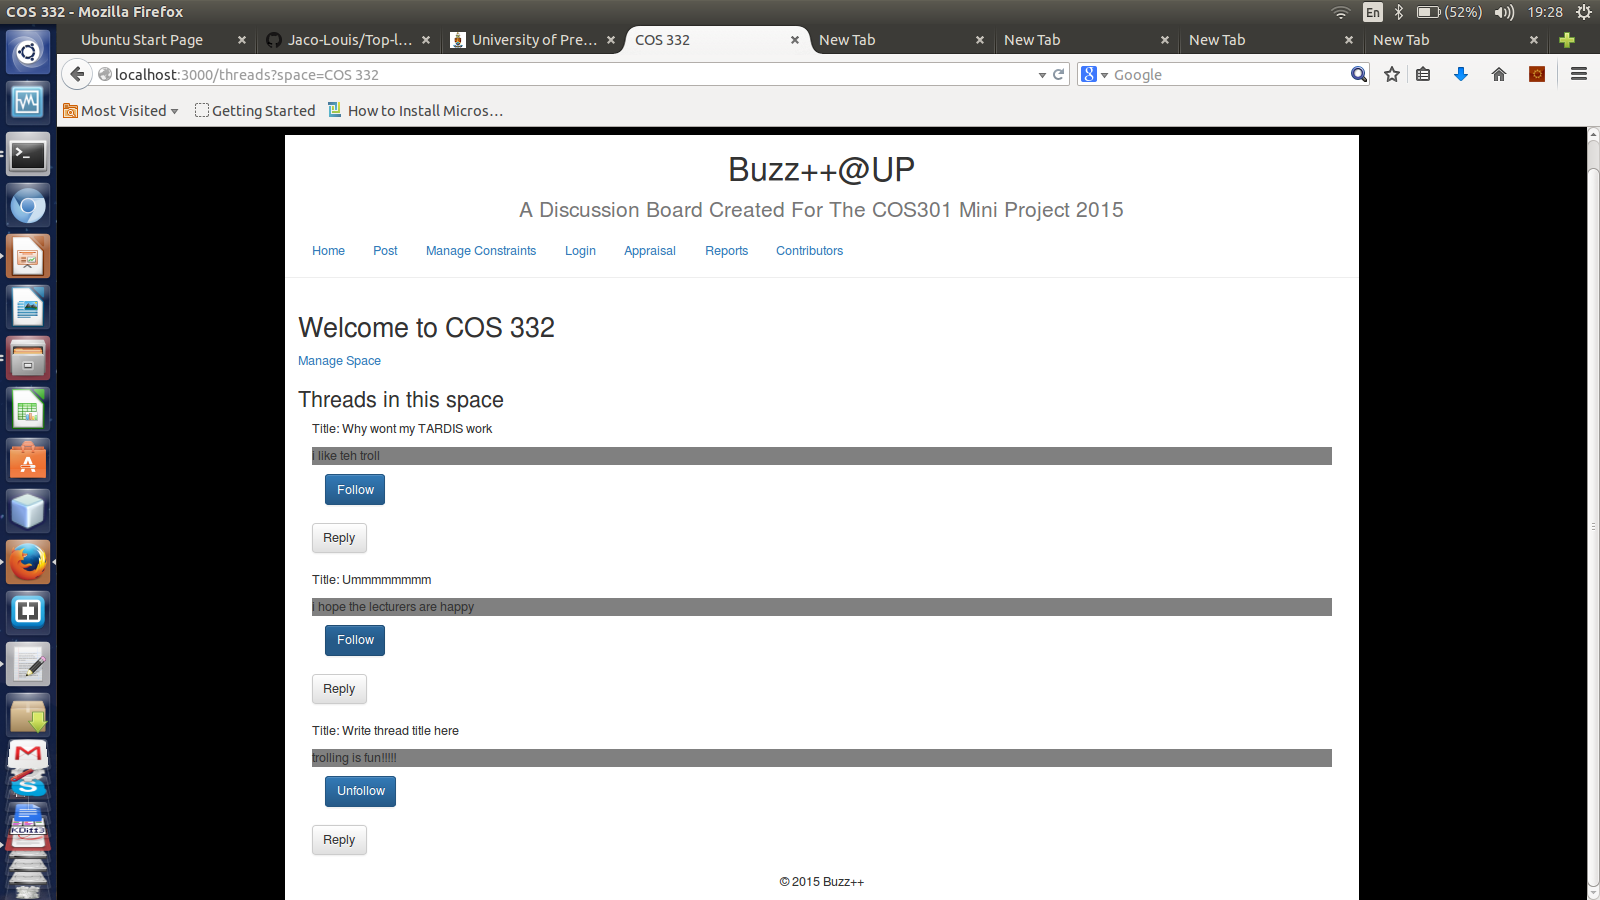
\includegraphics[width=0.85\textwidth]{UsabilityExplanatoryButtons} 
\end{figure}

Larger headings are used to label the different sections, for example under the Manage Constraints tab there are large headings to indicate the Existing constraints section and the Add new constraint section. This again contributes to ease of use for the novice first year user.

Through these mechanisms the system is memborable hence it is also be understandable.  

\item Integratibility:

The system is able to address future integration requirements by providing access to its services using widely adopted public standards such as firstly having separate npm packages for all the different modules. The packages are stored on Synopia. Also, electrolyte is being used in the server to provide a dependency injection. The HandleBars server is the main server that needs to be used to test and integrate all the modules on. The routes/index.js, routes/infrastructure.js and routes/content.js files use express to route the different hbs files for the different modules in order to integrate the infrastructure and content subsystems into the main system. 

\begin{figure}[h!]
  \centering
    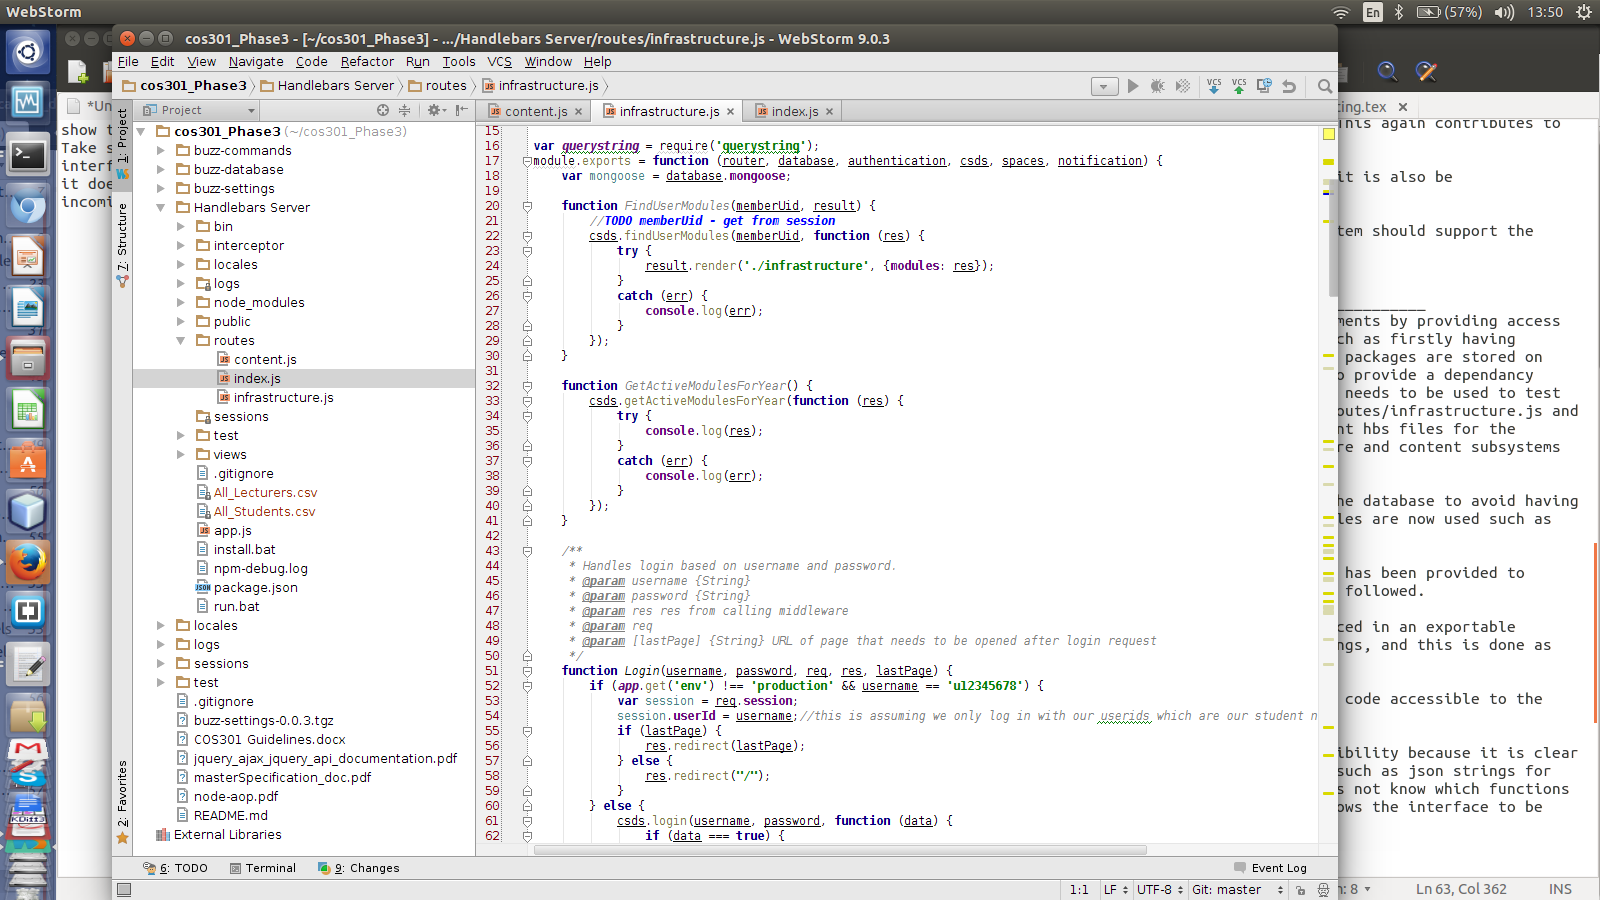
\includegraphics[width=0.85\textwidth]{IndexContentInfra} 
\end{figure}

\begin{figure}[h!]
  \centering
    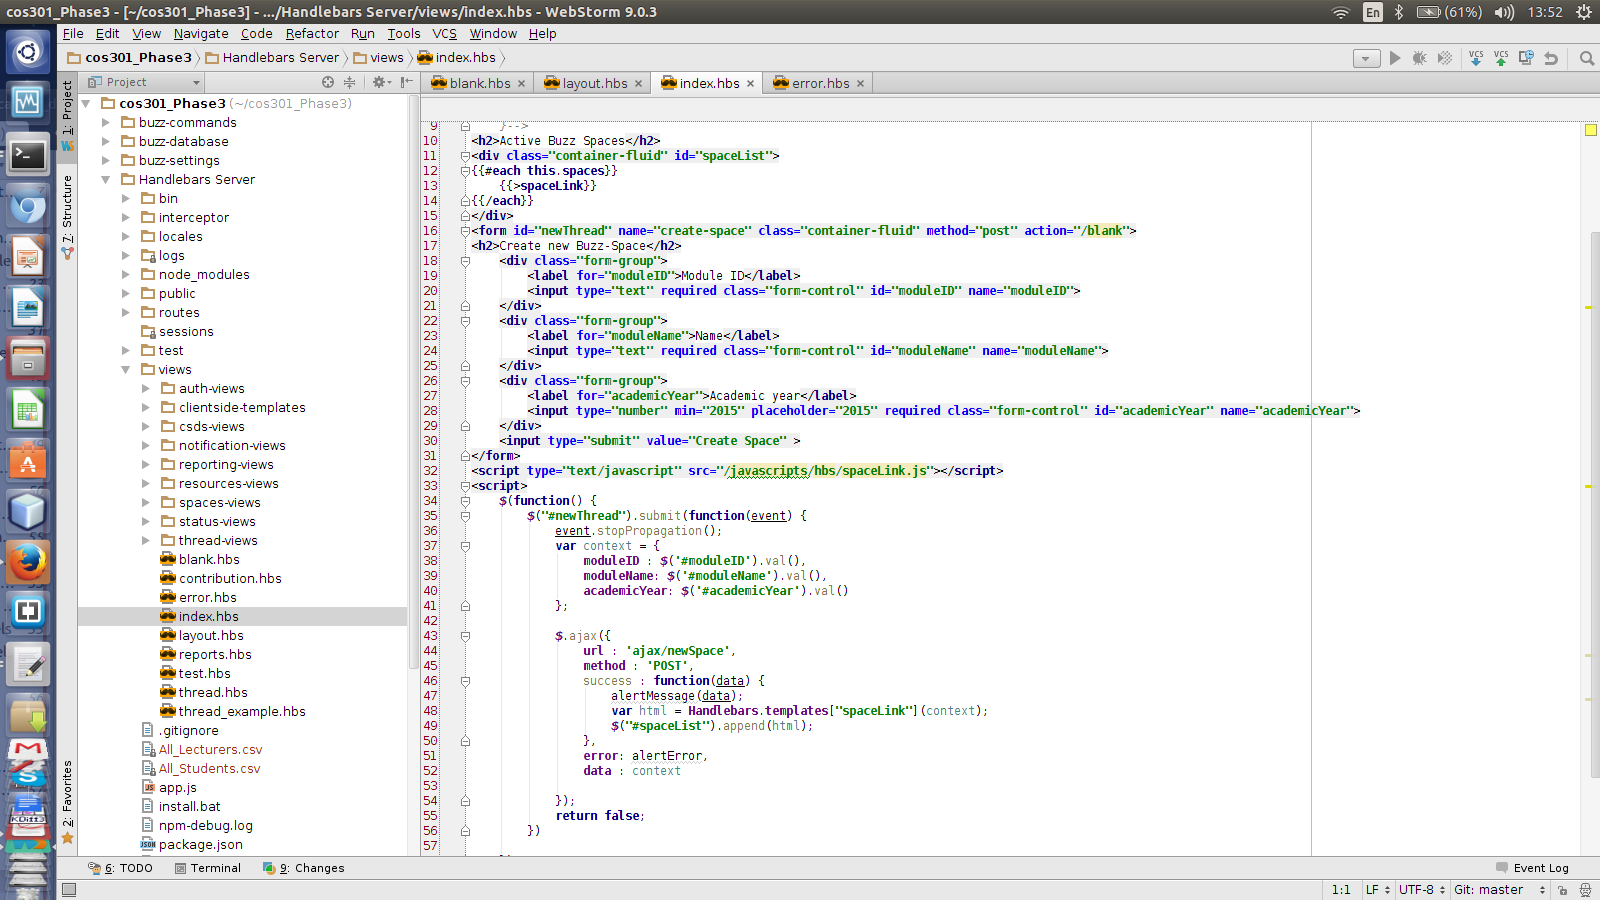
\includegraphics[width=0.85\textwidth]{HbsFiles} 
\end{figure}

A separate file is used to establish the connection to the database to avoid having this done in all the separate files. Also, global variables are now used such as the global password and username for example. 

A document has been provided via email and a README file has been provided to specify important standards and regulations that must be followed.

The functional code in the separate packages must be placed in an exportable function taking parameters such as the database or settings, and this is done as part of the electrolyte dependency injection. 

Exports are also used in the different files to make the code accessible to the other files.

The following screenshot indicates the systems' integratibility because it is clear that the following function is able to accept standards such as json strings for objects. This is intergrateble because the interface does not know which functions are sending the aforementioned objects. Therefore it allows the interface to be connected to any backend system.

\begin{figure}[h!]
  \centering
    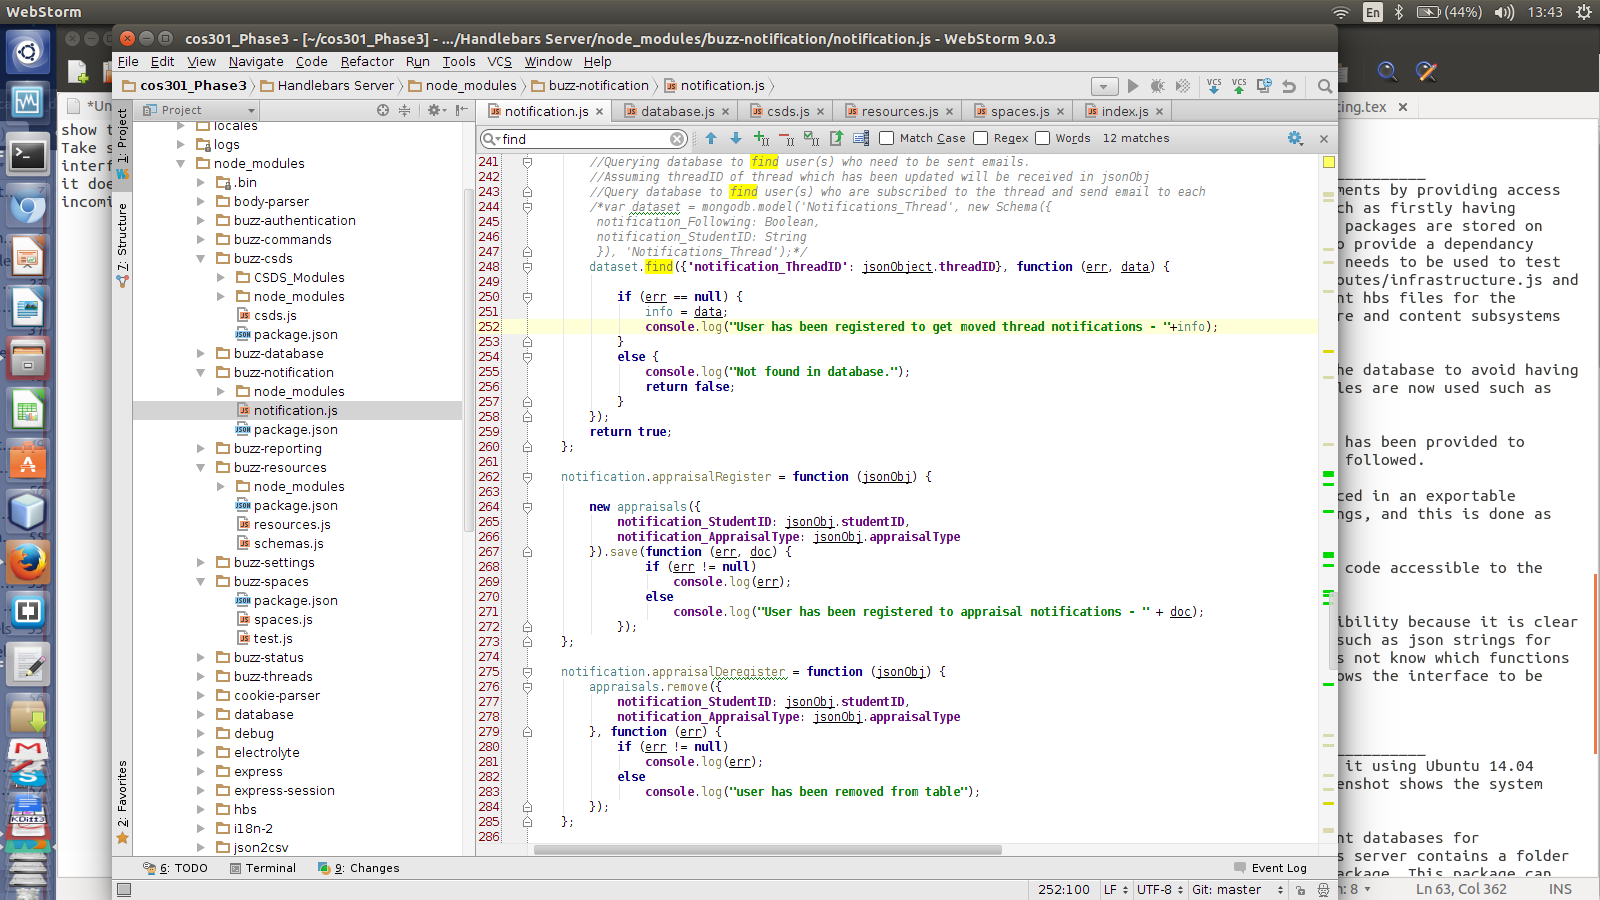
\includegraphics[width=0.85\textwidth]{JsonObject} 
\end{figure}


\item Deployability:

The system is deployable on Linux servers as we have run it using Ubuntu 14.04 Linux and the system was able to run. The following screenshot shows the system running on a Linux server:

\begin{figure}[h!]
  \centering
    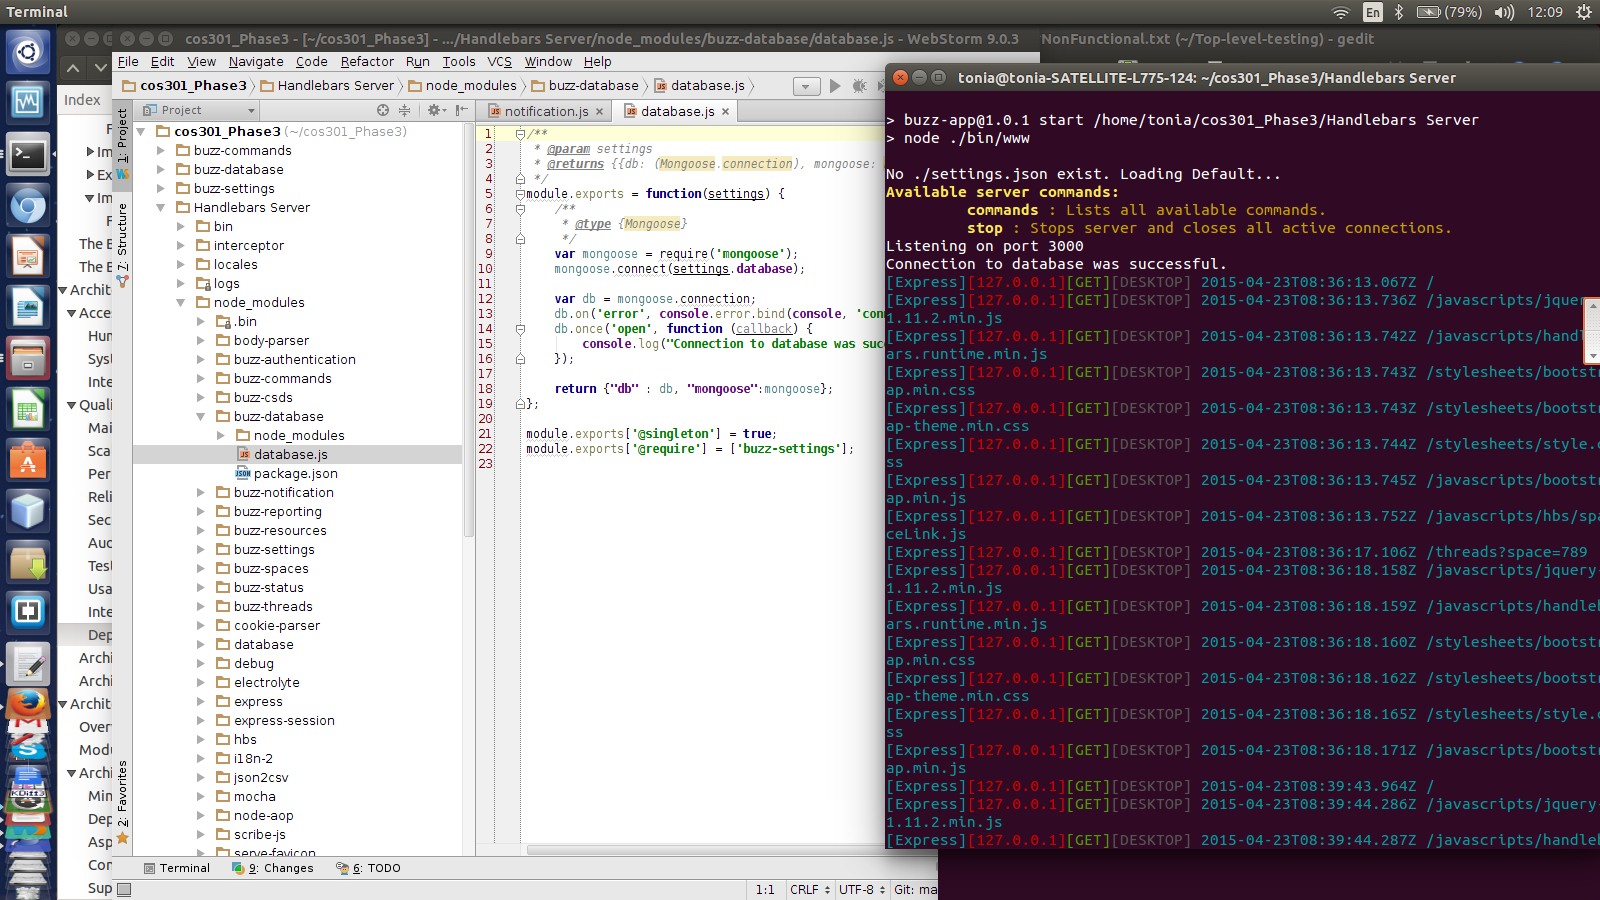
\includegraphics[width=0.85\textwidth]{LinuxServerScreenShot} 
\end{figure}

The system is deployable on an environment using different databases for persistence of the Buzz database because the Handlebars server contains a folder called node\_modules, and it contains the buzz\_database package. This package can easily be swapped out and an alternative database package can be plugged in, that the system can use due to the flexibility of this server. As long as the new package has the same name so that the files that require the database do not need to be changed, no major changes will need to be made.  
 

\begin{figure}[h!]
  \centering
    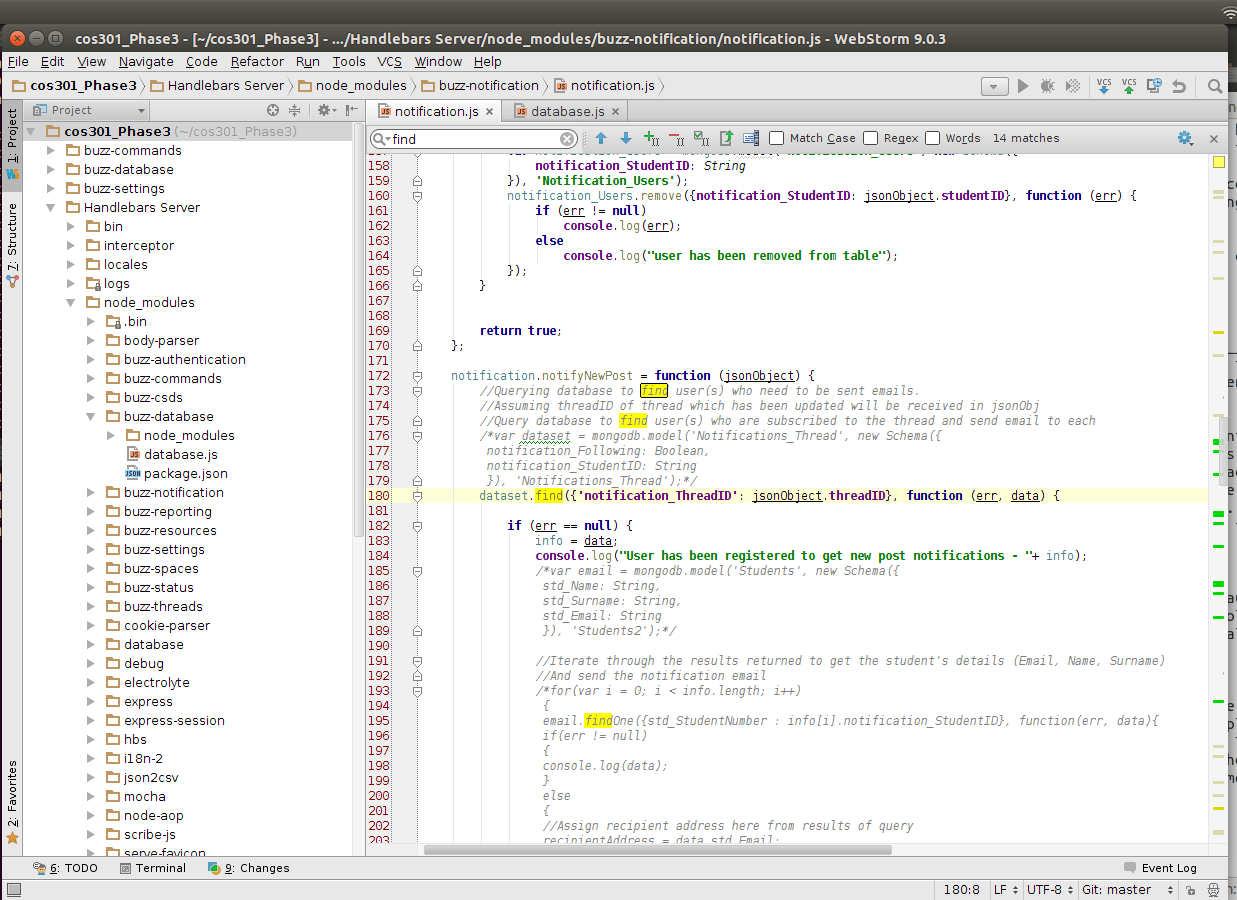
\includegraphics[width=0.85\textwidth]{DatabaseSchema} 
\end{figure}

\begin{figure}[h!]
  \centering
    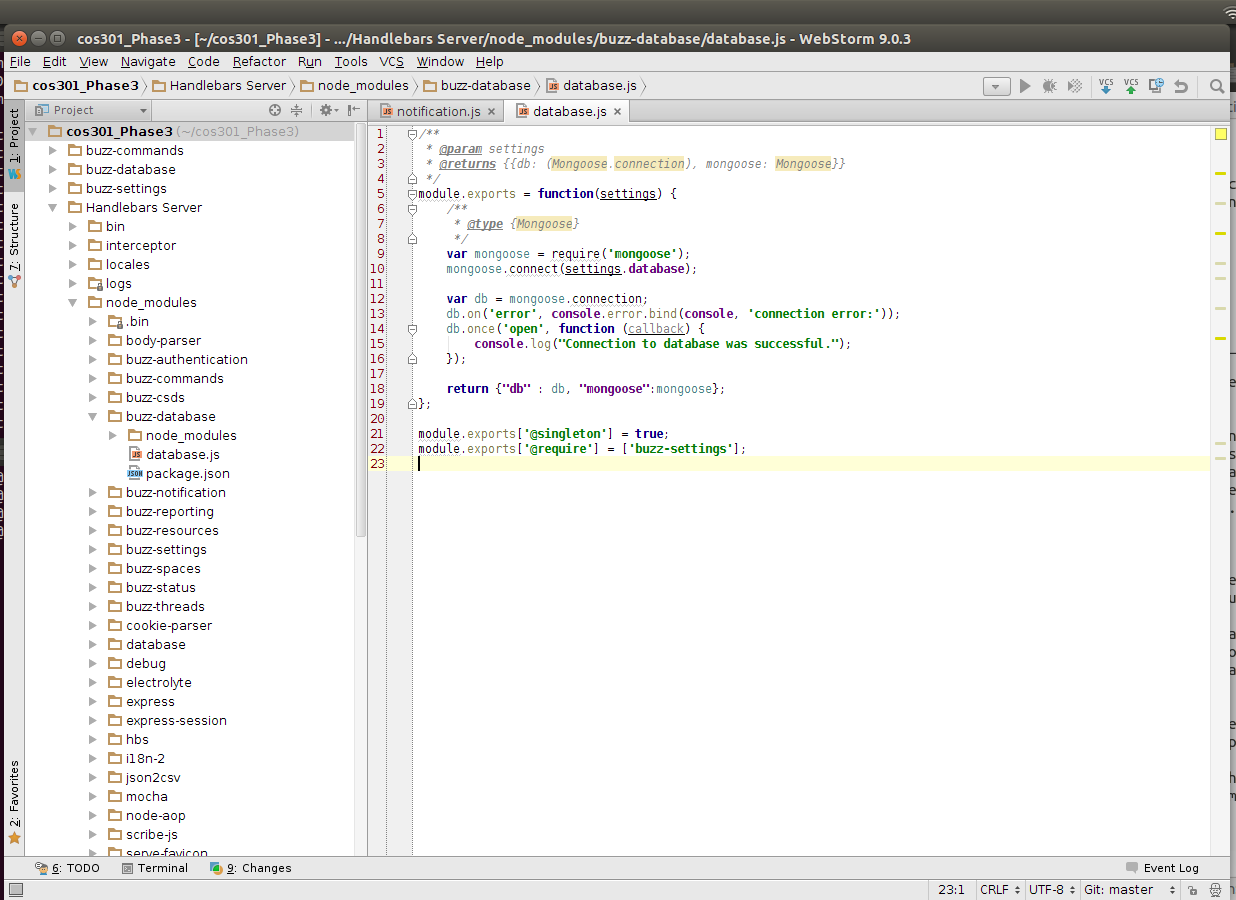
\includegraphics[width=0.85\textwidth]{databaseCurrent} 
\end{figure}

The system is deployable in environments where the user authentication credentials and roles are sourced from different repositories. The following screenshot indicates that the Handlebars server contains a folder called node\_modules, and it contains the buzz\_csds package. 


\begin{figure}[h!]
  \centering
    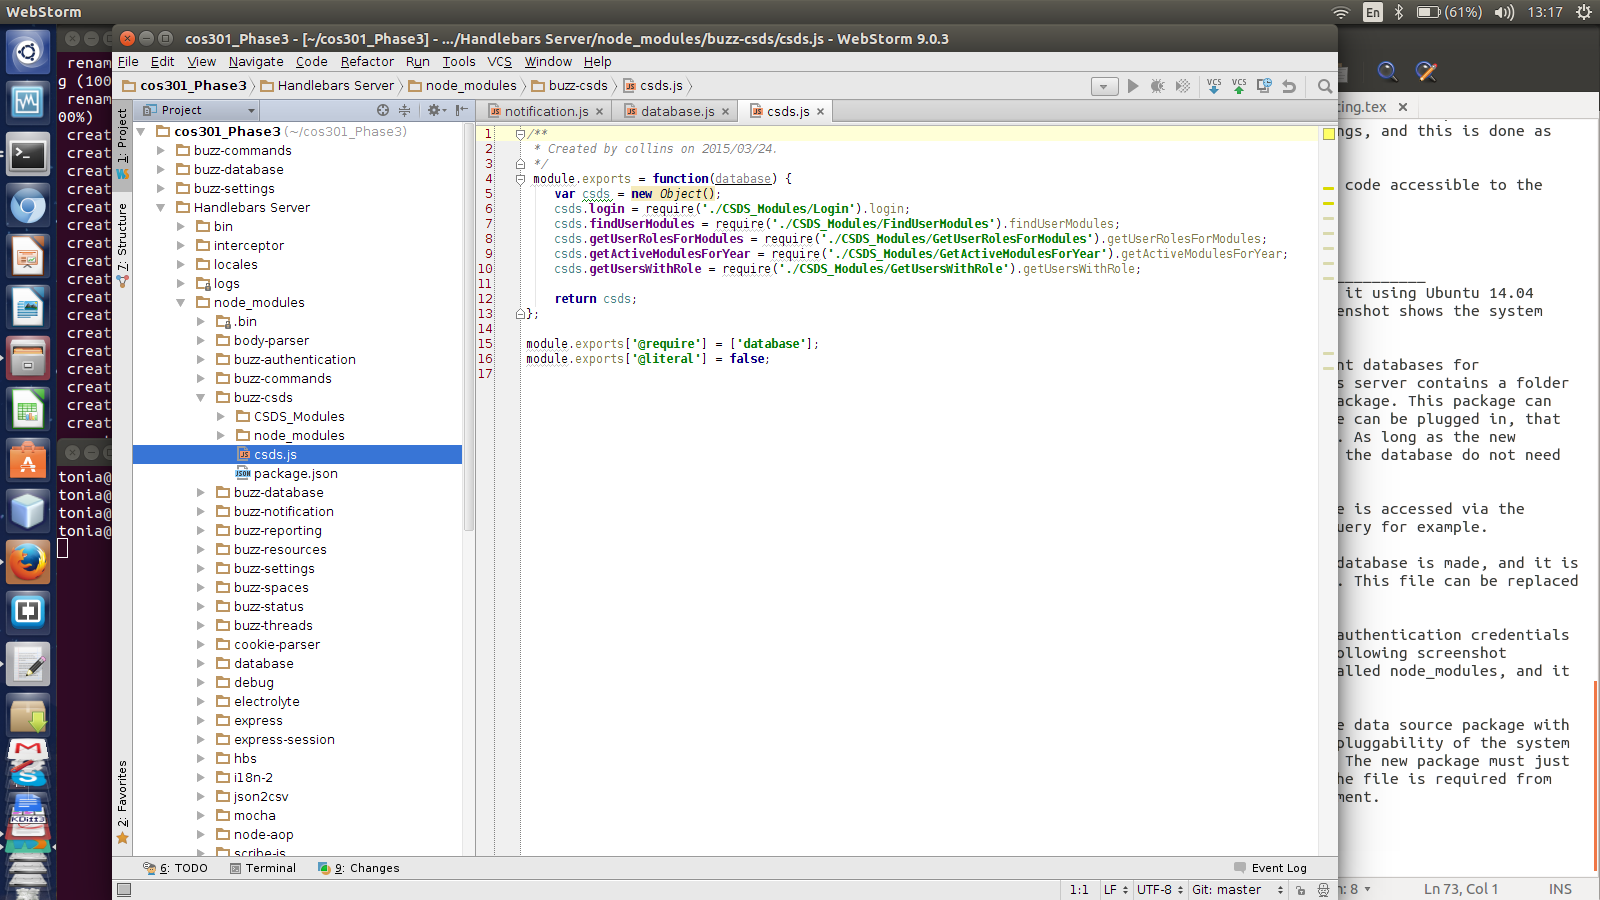
\includegraphics[width=0.85\textwidth]{CSDSPackage} 
\end{figure}
 
This package can easily be swapped out and an alternative data source package with different credentials and roles can be used, due to the pluggability of the system and dependency injection employed by the top level team. The new package must just be named the same as the old one to avoid errors where the file is required from the package in the code. 

\end{enumerate}


\subsection{Top Level B Testing Results}

\subsubsection{Functional Testing}

\begin{enumerate}
\input{authorizationB}
\item Buzz Resources Module

\textbf{Description}
	
The system suppose to integrate a resource module that is used to upload and manage resources like media files and documents that can either linked or embedded to a post.
	
\textbf{Preconditions}
\begin{itemize}
	\item Size constraints must be met
	\item The resource mimetype must be detected
	\item The resource to must be supported
\end{itemize}

\textbf{Post-conditions}
\begin{itemize}
\item Url for resource must be generated
\item Resource must persist
\end{itemize}

\textbf{Test Results}

The Buzz resources module works when test in isolation through unit testing but fails on automated integration testing, it was not integrated as required by system specification. 



		 		 
\item Buzz Notification Module

\textbf{Description}

This module is focused on registering for notification messages, for submitted threads and the posting of a particular user and any possible notification that one can receive for their posts via email.
 	
\textbf{Preconditions}
\begin{itemize}
	\item User must have registered to receive notifications 
\end{itemize}

\textbf{Post-conditions}
\begin{itemize}
\item User should receive all notification based on the domain (received from all threads or a particular thread) the user registered for to receive notifications.   
\end{itemize}

\textbf{Test Results}

The Buzz notification was not integrated for this system, no email notifications are sent when a thread or post is submitted. 
\item Buzz-Status module
	
The Buzz-Status module was expected to at least implement these 6 functional processes:
	
\begin{enumerate}
	\item assessProfile:
	\begin{itemize}
		\item\textbf{Objective: } Serve as a general interface through which lecturers can choose a pluggable implementation with which to assess user profiles.
		\item\textbf{Pre-conditions: } Have some form of administrative users and general users. It should also have profiles for users of the Buzz system. 
		\item\textbf{Post-conditions: } ProfileAssessor can return the queried information about a the profile of a user, according to various criteria but iy should, as a minimal requirement, at least be able to calculate the user’s status (i.e. the user’s rating).
		\item\textbf{Testing: } Although both pre-conditions were met, no actual implementation for this functional requirement is present in the Buzz system (meaning post-conditions were not met).
	\end{itemize}
\item setStatusCalculator:
	\begin{itemize}
		\item\textbf{Objective: } An interface through which a StatusCalculator can be assigned. The StatusCalculator is used to assign a status value to a user according to specific criteria. The default StatusCalculator should be NumPostAssesor which assigns a status directly proportional to the number of posts a user has made.
		\item\textbf{Pre-conditions: } It should have some form of administrative and general users. It should have profiles for users of the Buzz system. It should have a space where users can post content (this is a pre-condition for the default StatusCalculator, i.e. NumPostAssessor).
		\item\textbf{Post-conditions: } The assigned StatusCalculator must be able to assign a status value to all users.
		\item\textbf{Testing: } Only the first two pre-conditions are met. Although there is a space where users can post content (i.e. http://buzz-codechat.rhcloud.com/spaces/) it does not fulfil any of its required functionality (i.e. can’t successfully post content, no thread handling). There is no implementation of a StatusCalculator present in the Buzz system, therefore no post-conditions were met.
	\end{itemize}
\item getStatusForProfile:
	\begin{itemize}
		\item\textbf{Objective: } A simple query which returns the user’s status.
		\item\textbf{Pre-conditions: } Have profiles for users of the Buzz system. Each user has a status.
		\item\textbf{Post-conditions: } The user’s status is returned.
		\item\textbf{Testing: } Only the first pre-condition is met (i.e. user’s do not have statuses). There is no way of storing a user’s status in the Buzz system, it therefore fails to meet the post-condition.
	\end{itemize}
\item createAppraisalType:
	\begin{itemize}
		\item\textbf{Objective: }  Be able to create a data structure by which posts can be graded/appraised (e.g. FunnyAppraisalType allows user to mark a post as Hilarious, Funny or Boring).
		\item\textbf{Pre-conditions: } Have a space were posts can be displayed.
		\item\textbf{Post-conditions: }Have a user created data structure which can then be used to appraise/rank a post.
		\item\textbf{Testing: } The pre-condition is not met as although a space for posts exists, none of the required functionality exist (e.g. being able to post new content in a thread). The post-conditions are not met as no functions in the Buzz system implements the required functionality.
	\end{itemize}
\item activateAppraisalType:
	\begin{itemize}
		\item\textbf{Objective: } Assign an appraisal type (which was created by createAppraisalType) to be used in a specific Buzz space for a specific period of time.
		\item\textbf{Pre-conditions: }  Have a space where posts can be displayed. Have a function(s) which implements createAppraisalType.
		\item\textbf{Post-conditions: }Be able to use user created appraisal types in a certain buzz space for a specific period of time.
		\item\textbf{Testing: }  Neither pre-conditions are met as the Buzz space does not function properly and no version of createAppraisalType was implemented. This function was not implemented which means no post-conditions were met.
\begin{figure}[h!]
  \centering
    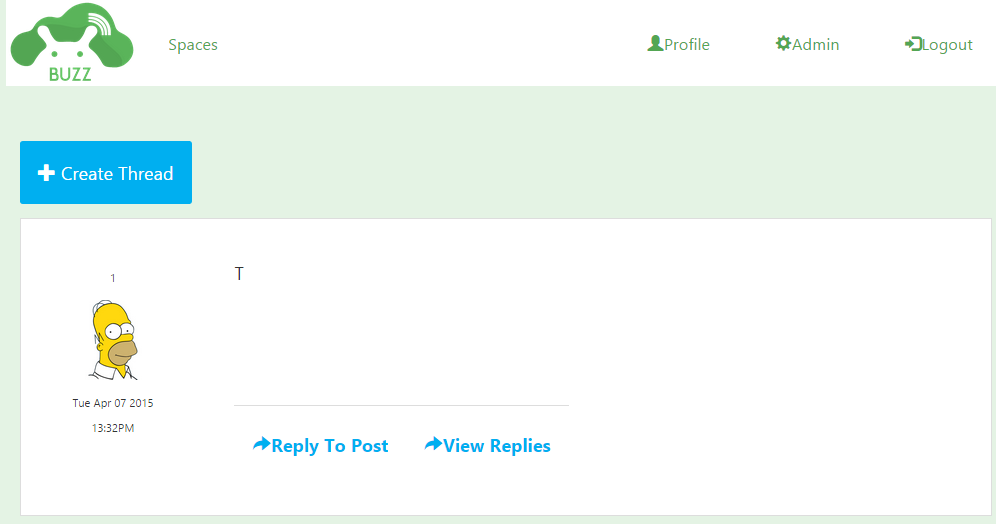
\includegraphics[width=0.85\textwidth]{No_appraisal}
    \caption{There are no appraisal icons that enables the user to "upvote" posts}
\end{figure}	
	\end{itemize}
\item assignAppraisalToPost:
	\begin{itemize}
		\item\textbf{Objective: } Allows the user to assign an appraisal to a post (i.e. rate a post).
		\item\textbf{Pre-conditions: }  Have a space where posts can be displayed.
		\item\textbf{Post-conditions: }The ranking/status of both the post and the user who posted the post will change.
		\item\textbf{Testing: } The pre-condition is not met as  the Buzz space does not function properly. This function was not implemented which means no post-conditions were met.
	\end{itemize}
\end{enumerate}
\item Buzz data source Module:

This module is responsible for sourcing data from the external cs database (Read Access) and using it for authentication and representation purposes.


\textbf{Use Cases}
\begin {itemize}


\item {Login and Administrative user}\\
This is the service that will authenticate against the cs data source where authentication credentials are stored

\begin {itemize}
\item Pre-conditions:\\
-should connect to CS data source (LDAP) (Not implemented-The system does not connect or acquire data from the computer science database )\\
        -user exists in ldap with provided authentication details (Implemented-The system has users that can connect to the system but are not in the cs data source, dummy users were created to provide the login functionality)\\
\item Post-conditions:\\
userID returned (not implemented-Code was found but no functionality)  
\end {itemize}

 
\begin{figure}[h!]
  \centering
    \reflectbox{%
      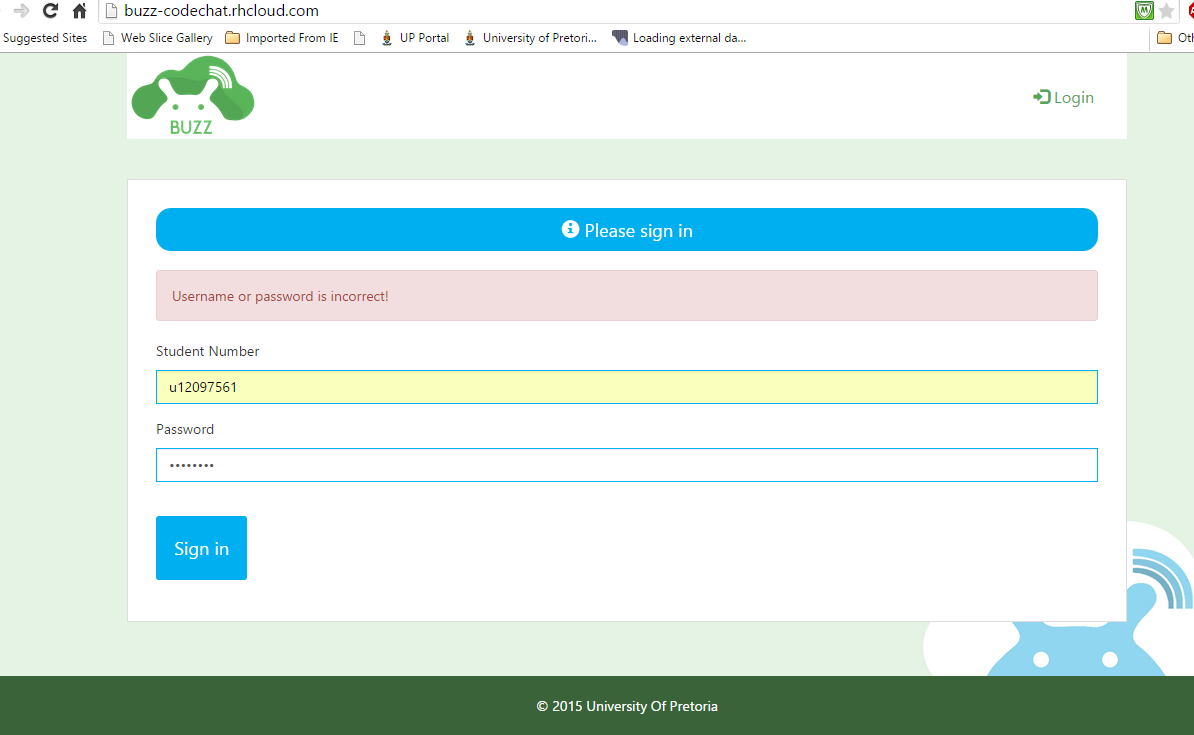
\includegraphics[width=0.5\textwidth]{loginadministrativeerror}}
  \caption{result to a user from the cs database trying to login }
\end{figure}


\begin{figure}[h!]
  \centering
    \reflectbox{%
      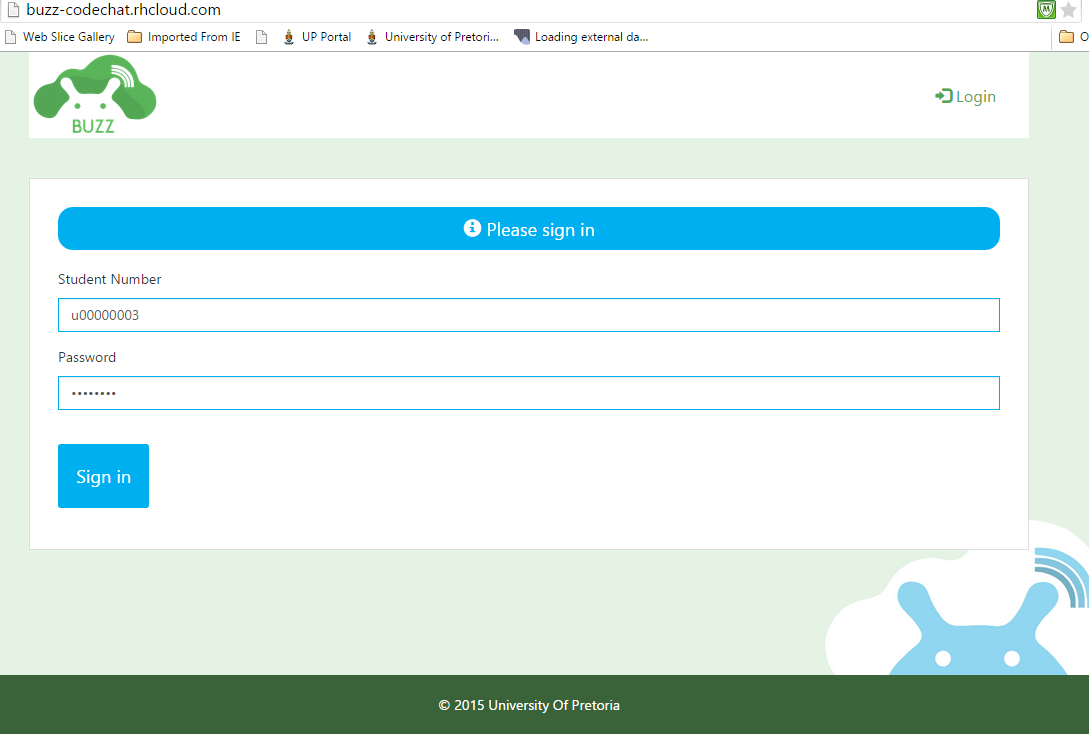
\includegraphics[width=0.5\textwidth]{loginadministrative(whatBdid)}}
  \caption{result to a dummy user not in the cs database trying to login }
\end{figure}

 
\item {getUsersRolesForModule}\\
This service is to query the user roles for a particular user\\


\begin {itemize}
\item Pre-conditions:\\
-should connect to CS data source (LDAP) (not implemented-No modules from cs data source where found , only one hard coded one)\\
        -user exists in ldap with provided authentication details (Not Implemented)\\
\item Post-conditions:\\
userID returned (not implemented)  
\end {itemize}


\begin{figure}[h!]
  \centering
    \reflectbox{%
      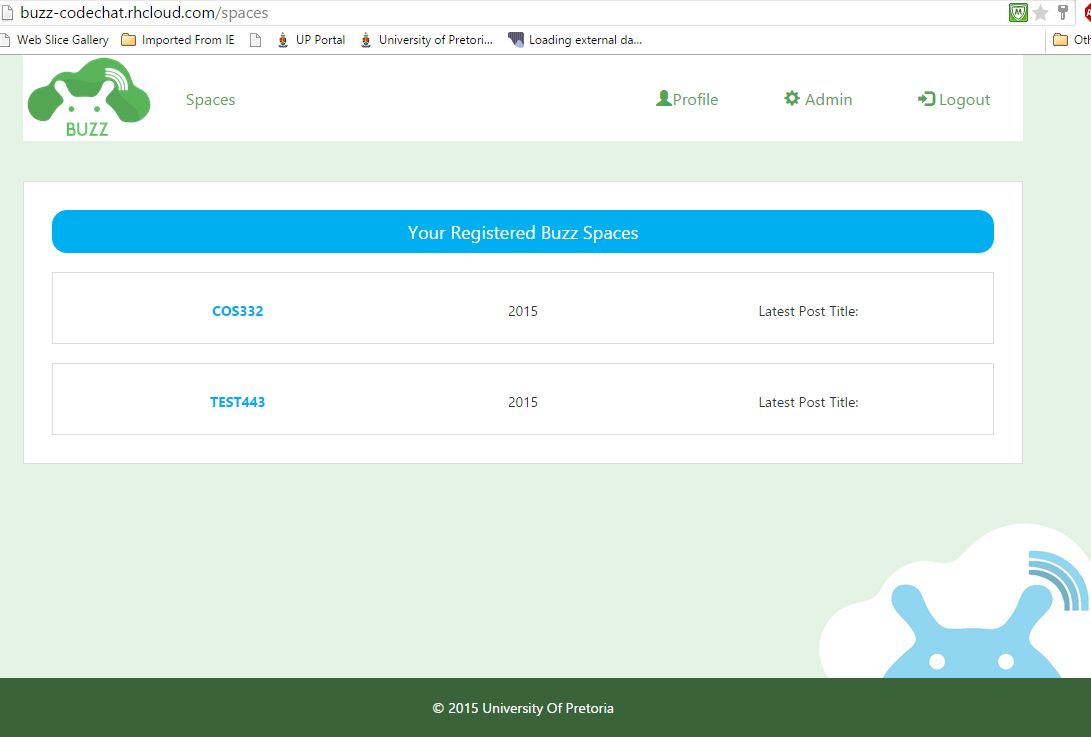
\includegraphics[width=0.5\textwidth]{modulesprovided}}
  \caption{result to a dummy user not in the cs database trying to login }
\end{figure}

 
\begin {itemize}
\item {GetUsersWithRole}\\
This service is required to retrieve al the users which have a role for a particular module
\\

\item Pre-conditions:\\
-should connect to CS data source (LDAP) (not implemented) No code found and no administrative users on site\\
 \begin{figure}[h!]
  \centering
    \reflectbox{%
      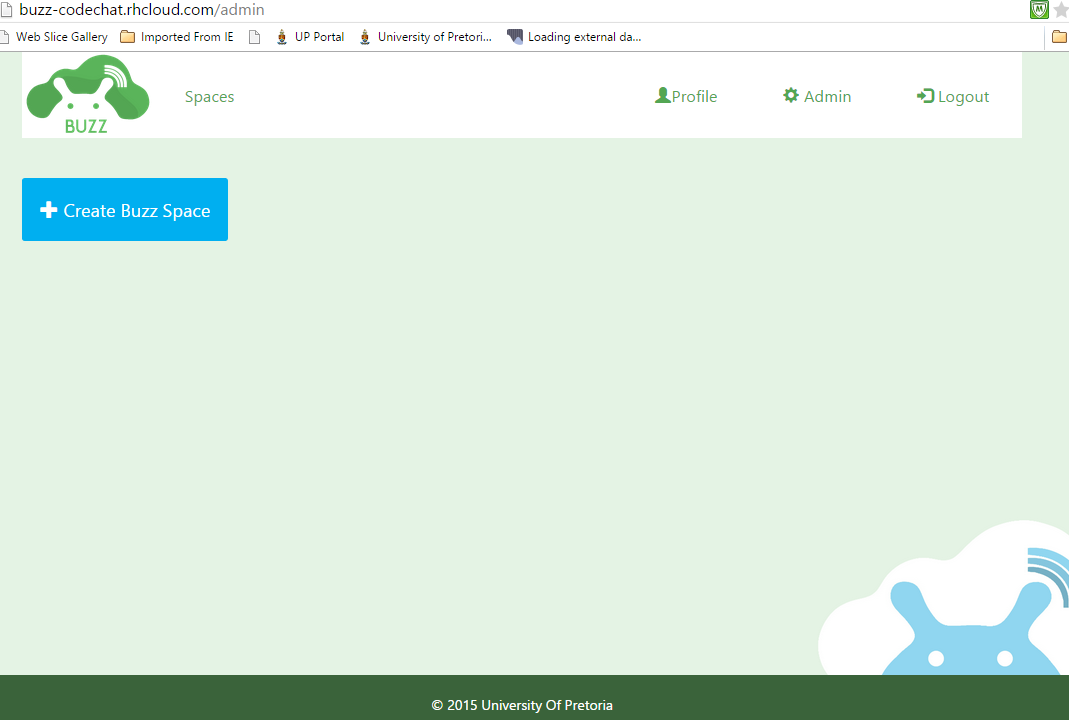
\includegraphics[width=0.5\textwidth]{userswithroles}}
  \caption{result to a dummy user not in the cs database trying to login }
\end{figure}   


 \end {itemize}  
\end {itemize}

\item  The Web Module:

The module provides a portal based, web responsive front end that allows a user to get access to the application facets.


\textbf{Sections}
\begin {itemize}


\item {Login/out}\\
The buzz system does allow user name u0000000n (with n being any single number starting from 1) and password "password" to login and out of the buzz system.

\begin{figure}[h!]
  \centering
    \reflectbox{%
      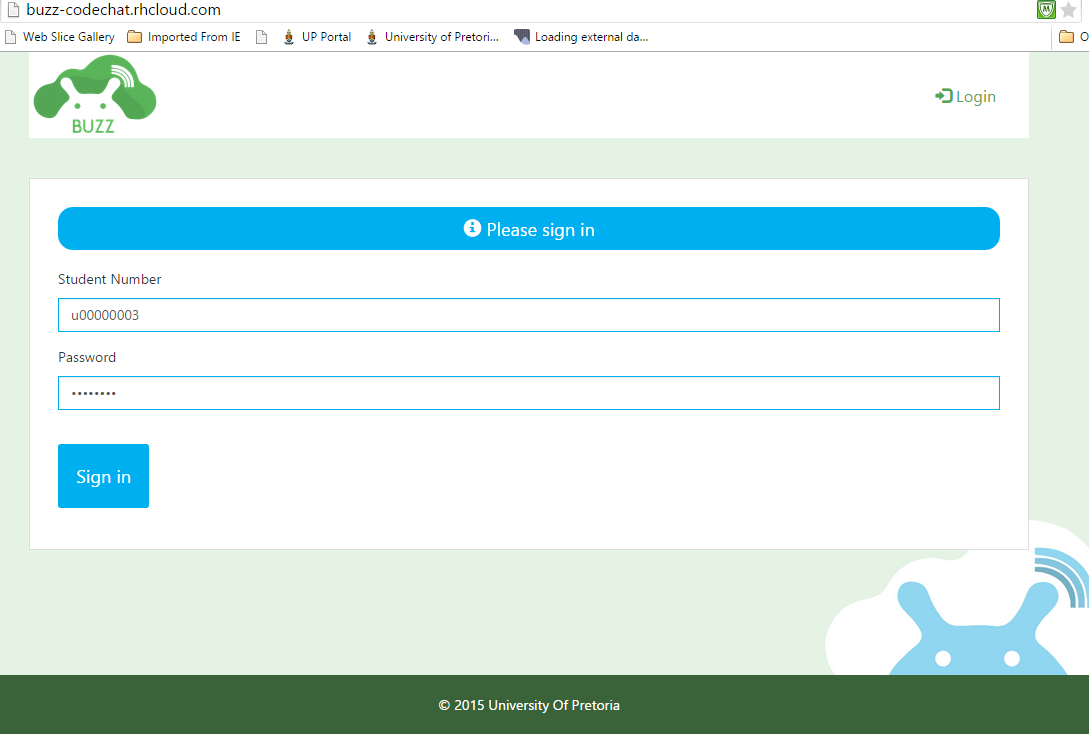
\includegraphics[width=0.5\textwidth,height=4cm]{loginadministrative(whatBdid)}}
  \caption{login format }
\end{figure}


\item personalization and configuration\\
A user cannot configure a dashboard type of view or buzz space, no functionality or options of such where provided.
\\

\item 	Accessibility of functionality\\
Access to a service does not depend on a user's role on a buzz space or a users status on that space, There is no form of grouping, all users are the same and have the same privileges and authorisations, basically all users have access to everything in the system.



\begin{figure}[h!]
  \centering
    \reflectbox{%
      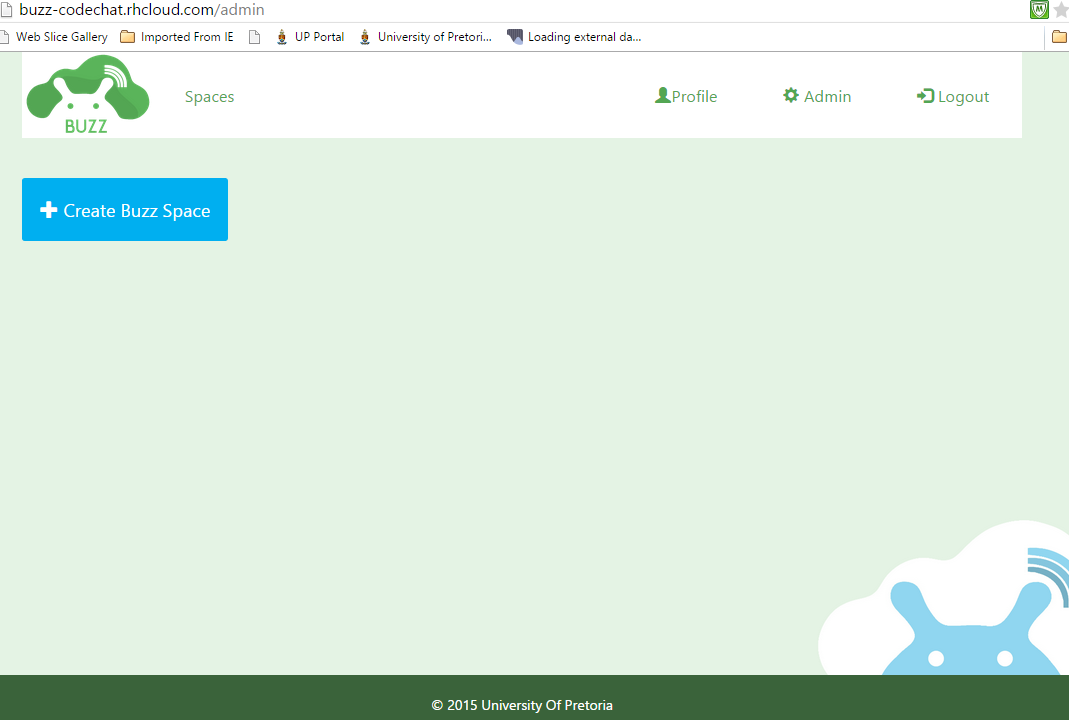
\includegraphics[width=0.5\textwidth,height=4cm]{userswithroles}}
  \caption{User roles in the system }
\end{figure}

\item {spaces}\\
In the buzz space, users are able to view the buzz spaces that are available, no clear distinction of modules registered for and modules they have not yet registered for is presented\\

\begin{figure}[h!]
  \centering
    \reflectbox{%
      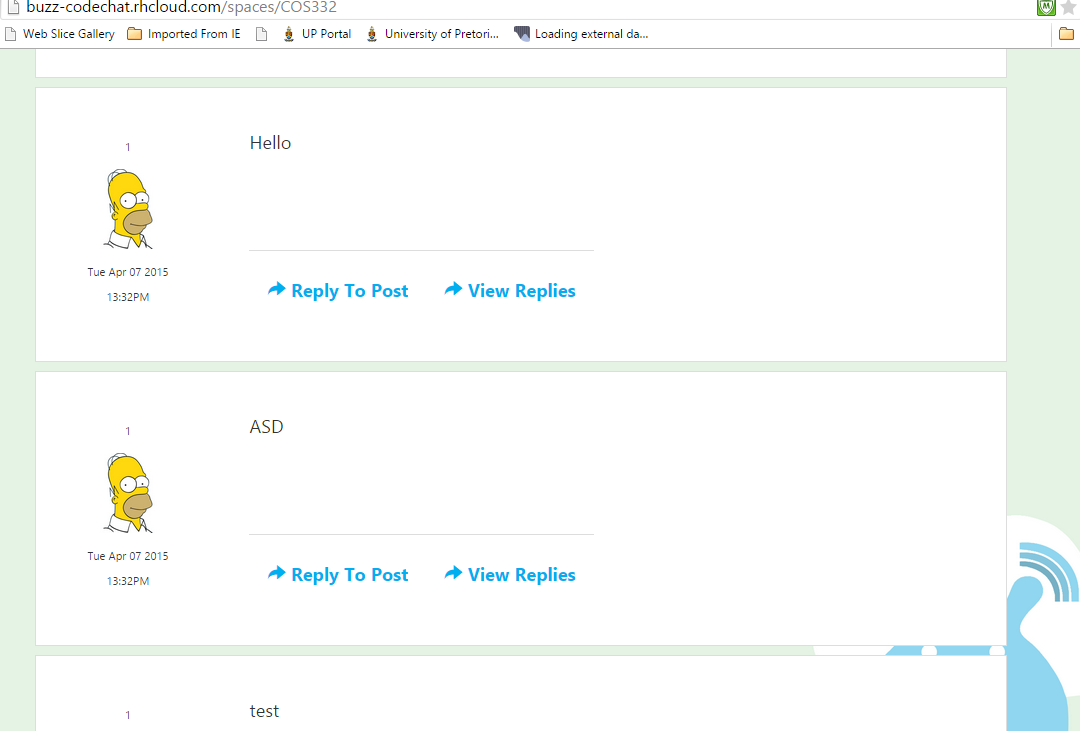
\includegraphics[width=0.5\textwidth,height=4cm]{threads}}
  \caption{threads on the space }
\end{figure}


\item 	UI Considerations around threads\\
Threads are posted as a flat list of posts showing the contents of each posts, no user can post; only view posts hard coded in to the system\\

\item	posts\\
Posts have header, content and footer area, in the buzz space the header contains the user name, the date/time and a profile picture of the user who submitted the post.  The footer contains the submission buttons, no appraisal values, no appraisal types and no posts can be submitted, created or replied to 

\begin{figure}[h!]
  \centering
    \reflectbox{%
      \includegraphics[width=0.5\textwidth,height=4cm]{repytoposterror}}
  \caption{error received when user tries to post }
\end{figure}

 

\item {profile information}\\
A user cab view their own profile picture and are given an option to upload a new one yet that functionality does not work, a user cannot view their user name, role of the user or status and the number of posts/appraisals made/received by the user
\\

 \begin{figure}[h!]
  \centering
    \reflectbox{%
      \includegraphics[width=0.5\textwidth,height=4cm]{dummyprofileprovided}}
  \caption{Dummy Profile data }
\end{figure}   


  
\end {itemize}

\item Buzz Reporting Module

\textbf{Description}
	
The reporting module provides services to gather, import and export information about posts in
specified subsets.


\textbf{Test Results}

The Buzz reporting module is not implemented thus cannot be tested.

\end{enumerate}

\subsubsection{Non-functional Testing} 

\begin{enumerate}
\item Maintainability:

The Buzz(B) system is maintainable in the following aspects:

\begin{itemize}
\item Understandable by future developers:

Every subsystem or 'module' of the system is implemented as a seperate functioning module.
Standalone modules are then plugged into the system.
New developers can change modules independantly.
\item Technologies used is current and expected to be available for a long time:

Node.js makes up the core of the buzz system. It is a widely used open-source platform released in Q1 of 2009. Popularity has grown tremendously and is not expected to stop growing in the near future. 

MongoDB is used as a database structure of the Buzz system and is highly compatible with Node.js. Also released in 2009 and is now the fourth most popular type of database management system.  MongoDB is expected to grow even more in the coming years which makes it   a good choice for the Buzz system in terms of maintainability.

\item The system is easily updated

New functionality can be added by adding modules to the system.
Functionality can be changed by changing independat modules without having to rebuild the whole system.
\end{itemize}
\item Scalability

The Buzz(B) system is partially scalable in the following aspects:

\begin{itemize}
\item Able to host buzz spaces for all Computer Science modules:

The Buzz(B) system failed this scalability test. It does not support functionality of adding a new buzz space thus cannot host buzz spaces fot all CS modules.

\item University-wide, servicing in the order of 50 000 students:

The Buzz(B) system failed this scalability test. It does not support functionality of adding a new user or student. Thus one default user exists as apposed to 50 000.
\end{itemize}
\newpage
\item Auditability:

\textbf{Description}

The system needs to log all requests and all responses for all user services provided
by the system.

\textbf{Test Results}

The figure below shows that the Buzz Space system is partially auditable, only the requests for the user serves of the system are logged. The logged request only contains:
\begin{itemize}
\item User serves requested.
\item Request object stringified as JSON
\end{itemize}

There are no log responses that are provided by the system, and the serves required to extract information from the audit logs is also not available not provided.

\begin{figure}[h]
  \centering
    \includegraphics[width=0.85\textwidth]{BuzzBAuditability}
    \caption{Buzz Space B Auditability Test}
\end{figure}

\newpage
\item Testability:

\textbf{Description}

A system needs testabl through:
\begin{itemize}
\item Unit testing components in isolation
\item Integration tests where the components are integrated to the actual environment
\end{itemize}

\textbf{Test Results}
   
The Buzz system is divided into manageable components (modules) for each use case. Breaking the system into these components makes make the system testable through unit testing using mock objects. The Buzz system is a modular system, the system components are pluggable and makes automated integration testing simple as the component is integrated in the entire system.    
\item Performance requirements:

Requirements for the Buzz system were for non-reporting operations to preferably not last longer than 0.2 seconds and for report queries to be processed in no more than 5 seconds.
To test this we used Firebug, an open source web browser extension of Firefox used for webpage monitoring. (Version used: Firebug 2.0.7).
The Buzz system met these requirement:
\begin{itemize}
\item Non-reporting operations such as returning to a previous page (i.e. operations that relied on cached copies of a webpage) completed relatively close to the target time limit (e.g. returning to the main Buzz Spaces page after viewing the user’s profile took only 0.286 seconds, very close to the target time of 0.2 seconds).

\begin{figure}[h!]
  \centering
    \includegraphics[width=0.85\textwidth]{Non-reporting_operationB}
    \caption{Non-reporting operation test}
\end{figure}

\item Report query operations (i.e. which had to communicate and receive some information from the system’s database) also completed within their desired time limit of 5 seconds (e.g. accessing the test module “TEST443”’s discussion space took only 1.24 seconds). Even some of the report query operations which took comparatively long to complete stayed within the 5 second limit (e.g. accessing module “COS332” took 4,81 seconds and accessing the Admin tab took 4,96 seconds).

\begin{figure}[h!]
  \centering
    \includegraphics[width=0.85\textwidth]{Reporting_operationB}
    \caption{Reporting operation test}
\end{figure}

\end{itemize}	

\item Reliability and availability:

\begin{itemize}
	\item textbf{Availability: }
	The Buzz system can be accessed at the following URL (http://buzz-codechat.rhcloud.com/) at any time of day on any of the widely used 	web browsers (Google Chrome, Mozilla Firefox, Microsoft Internet Explorer, Safari and Opera). The Buzz system even functions and displays 	correctly on the web browsers of mobile devices to ensure maximum availability.
	\item textbf{Reliability: }
	The system performs various error checks to ensure that no user action could cause the Buzz system to fail/crash (e.g. returning error messages if the user tries to log on with incorrect information , Figure 3). Even in cases were the system’s functionaity was not fully implemented procedures are in place to rather warn the user of incomplete operations instead of blindly carrying out a harmful request (e.g. an error message is diplayed when a user tries to upload a new profile picture, Figure4). The reason why the Buzz system can still function (to an extent) even though much of its functional procedures are incomplete/missing is due to the modular fashion in which the system was created. Even if one module of the system fails it is appropriatley seperated from the other modules to prevent a complete system failure.

\begin{figure}[h!]
  \centering
    \includegraphics[width=0.85\textwidth]{ReliabilityB1}
    \caption{Login error}

\begin{figure}[h!]
  \centering
    \includegraphics[width=0.85\textwidth]{ReliabilityB2}
    \caption{Error when uploading new profile picture}
\end{itemize}
	

\item {Integratibility:}\\

The system uses separate npm packages for each module which make it easy to share, update and reuse the code and hence integrate-able.  
\item {Deployability:}\\

The System is Deployable on both Linux and windows servers as it was run and worked fine in both cases, the following screen shot shows the system running on a windows server.
\end{enumerate}

\newpage
\section{Conclusion}

The Buzz systems had been tested, evaluated and compared to the original specification that defined how the system should be implemented. The evaluation of both implementations have brought up several interesting facets. It has been noted that both systems function to an extent, but none of the two implementations fulfilled the requirements completely. The systems implemented showed some promise in terms of some modules when viewed in isolation, while some modules did not function completely. Some modules failed to satisfy testing requirements such as unit tests, while others excelled at their unit tests. The integration of several related modules led to great success while others failed. At the top level some implementations delivered a well-functioning system, but lacked in terms of security and completeness. The other implementation led to a well functioning interfaced system, but lacked in terms of functionality. The testing of both systems led to the conclusion that the systems both worked to some extent, but failed to satisfy the complete requirements of the original specification of the system.

\end{document}
